% SPDX-FileCopyrightText: (c) 2026 Tim S. B. (GitHub: cpldcpu)
% SPDX-License-Identifier: Apache-2.0
\documentclass[10pt,a4paper]{article}

\usepackage[T1]{fontenc}
\usepackage[utf8]{inputenc}
\usepackage[margin=17mm, top=18mm, bottom=15mm]{geometry}
\usepackage{lmodern}
\usepackage{microtype}
\usepackage{amsmath,amssymb}
\usepackage{graphicx}
\usepackage{booktabs}
\usepackage{tabularx}
\usepackage{array}
\usepackage{multirow}
\usepackage{colortbl}
\usepackage{xcolor}
\usepackage{tikz}
\usetikzlibrary{arrows.meta,positioning,fit,backgrounds,calc}
\usepackage{listings}
\usepackage{fancyhdr}
\usepackage{float}
\usepackage{hyperref}

\definecolor{AccentBlue}{HTML}{154C79}
\definecolor{SoftBg}{HTML}{F4F7FA}
\definecolor{PassGreen}{HTML}{1B5E20}
\definecolor{PassBg}{HTML}{E8F5E9}
\definecolor{WarnAmber}{HTML}{8D4E00}
\definecolor{CodeBg}{HTML}{F7F7F7}

\hypersetup{
  colorlinks=true,
  linkcolor=AccentBlue,
  urlcolor=AccentBlue,
  pdftitle={rpe_clk_analog: Custom Analog Clock Macro Design Report (IHP SG13CMOS5L)},
  pdfauthor={Antigravity (Design & Report); Project Owner: Tim}
}

\pagestyle{fancy}
\fancyhf{}
\lhead{\small\textcolor{AccentBlue}{\texttt{rpe\_clk\_analog}} Custom Analog Clock Macro --- IHP \texttt{sg13cmos5l}}
\rhead{\small Design \& Physical Sign-Off Report}
\cfoot{\small Page \thepage}
\renewcommand{\headrulewidth}{0.4pt}

\lstset{
  basicstyle=\ttfamily\footnotesize,
  backgroundcolor=\color{CodeBg},
  frame=single,
  rulecolor=\color{gray!40},
  breaklines=true,
  columns=fullflexible
}

\setlength{\parskip}{0.36em}
\setlength{\parindent}{0pt}

\begin{document}

% =============================================================================
% TITLE BLOCK
% =============================================================================
\begin{center}
  {\LARGE\bfseries\color{AccentBlue} Custom Dual-Oscillator Analog Clock Macro (\texttt{rpe\_clk\_analog})\\[3pt]
  Architecture, Circuit Design, Physical Layout \& Sign-Off Report}\\[6pt]
  {\normalsize\bfseries Design \& Report: Antigravity \quad|\quad Project Owner: Tim}\\[3pt]
  {\normalsize Process: IHP \texttt{ihp-sg13cmos5l} ($130\text{ nm}$ CMOS5L, $1.20\text{ V}$ core / $3.3\text{ V}$ TGO) \quad|\quad
  Tools: \texttt{xschem}, \texttt{ngspice}, KLayout 0.30.12, Magic 8.3.677}
\end{center}
\vspace{0pt}

\begin{abstract}
\noindent This report documents the end-to-end design, characterization, compacted custom physical layout, parasitic-aware re-centering, DRC/LVS sign-off, and hierarchical Magic 8.3.677 parasitic extraction (PEX) of \texttt{rpe\_clk\_analog}, a unified analog clock-generation macro for the Changeling-Alpha SoC in IHP \texttt{ihp-sg13cmos5l}. The macro integrates two independent oscillators sharing a single $0.5\,\mu\text{A}$ self-biased startup reference (\texttt{bias}): (1) a 5-stage CMOM-loaded current-controlled ring oscillator (\texttt{osc\_ring\_cc}) driven by an 8-bit segmented thermometer+binary current DAC (\texttt{idac\_8b}) co-optimized against post-layout parasitics ($2.4\times 2.4\,\mu\text{m}$ \texttt{cap\_cmomf}, $w=1.5\,\mu\text{m}$ master PMOS, and non-inverting stage routing), yielding $15.84$--$83.77\text{ MHz}$ at \texttt{tt} ($59.92\text{ MHz}$ at \texttt{trim=155}, $48.74\%$ duty cycle, $61.50\,\mu\text{A}$) and covering the $60\text{ MHz}$ target across \texttt{tt}/\texttt{ss}/\texttt{ff} ($78.08$--$96.89\text{ MHz}$ max) while keeping default boot \texttt{trim=128} $\le 60\text{ MHz}$ across all corners ($52.78 / 52.98 / 58.51\text{ MHz}$) in full Magic PEX; and (2) an ultra-low-power dual-slope relaxation oscillator (\texttt{relax\_core}) combining a $4\times\text{rppd}$ poly-resistor threshold reference with dual HV \texttt{SVaricap} ($N_x=8$) integrating capacitors and \texttt{nmosHV} reset switches to synthesize $98.54\text{ kHz}$ post-layout ($112.07\text{ kHz}$ schematic) at $4.15\,\mu\text{A}$ active macro current. Shared \texttt{en\_or} power gating limits post-layout deep-standby leakage to $6.05\text{ nA}$ (\texttt{tt}) and $68.68\text{ nA}$ (\texttt{ss}, $125\,^\circ\text{C}$). After subblock compaction and parasitic re-centering inside a 2-column floorplan, the custom layout occupies $171.500 \times 137.000\,\mu\text{m}$ ($23{,}495.5\,\mu\text{m}^2$, $-42.1\%$ vs.\ initial $40{,}592.0\,\mu\text{m}^2$) and passes IHP KLayout DRC (\texttt{main} and \texttt{main antenna}: $0$ violations), strict-port LVS (\texttt{Congratulations! Netlists match.}, $211$ combined devices across $117$ nets, $14/14$ ports matched), and full $3{,}607$-capacitor ($1{,}334.46\text{ fF}$) hierarchical Magic PEX closure.
\end{abstract}

\begin{table}[H]
\centering
\caption{Executive Summary of Verified \texttt{rpe\_clk\_analog} Specifications (\texttt{ngspice} Schematic/PEX \& KLayout Sign-Off).}
\label{tab:exec_summary}
\small
\begin{tabularx}{\textwidth}{@{}ll >{\raggedright\arraybackslash}X@{}}
\toprule
\textbf{Parameter} & \textbf{Verified Value} & \textbf{Condition / Evidence Source} \\
\midrule
Process / Supply & IHP \texttt{ihp-sg13cmos5l}, $1.20\text{ V} \pm 10\%$ & Core $1.08$--$1.32\text{ V}$, $-40$ to $125\,^\circ\text{C}$; HV \texttt{TGO} for \texttt{SVaricap}/\texttt{nmosHV} \\
Compacted Macro Footprint & $171.500 \times 137.000\,\mu\text{m}$ ($23{,}495.5\,\mu\text{m}^2$) & $-42.1\%$ vs.\ initial $40{,}592.0\,\mu\text{m}^2$ (\texttt{rpe\_clk\_analog.gds/.lef}) \\
Fast Clock (\texttt{clk}) Range (PEX) & $15.84$--$83.77\text{ MHz}$ (\texttt{tt}, \texttt{trim} $0$--$255$) & \texttt{clk\_macro\_pex\_trim.csv}; \texttt{ss} $17.32$--$78.08$, \texttt{ff} $16.99$--$96.89\text{ MHz}$ \\
Nominal $60\text{ MHz}$ Point (PEX) & $59.92\text{ MHz}$, $48.74\%$ duty, $61.50\,\mu\text{A}$ & Post-layout \texttt{ring\_only} (\texttt{tt}, $1.20\text{ V}$, $25\,^\circ\text{C}$, \texttt{trim=155}) \\
Boot-Safe Default (\texttt{trim=128}, PEX) & $52.78$ (\texttt{tt}), $52.98$ (\texttt{ss}), $58.51\text{ MHz}$ (\texttt{ff}) & Always $\le 60\text{ MHz}$ post-layout across \texttt{tt}/\texttt{ss}/\texttt{ff} (\texttt{clk\_macro\_pex.csv}) \\
Pre-Emphasized Ring (Sch.) & $35.14$--$193.63\text{ MHz}$ ($136.39\text{ MHz}$ @ \texttt{155}) & \texttt{osc\_ring\_cc\_trim.csv}; $-45.0\%/\text{V}$ supply slope @ \texttt{trim=38} \\
Slow Clock (\texttt{clk\_slow}, PEX) & $98.54\text{ kHz}$, $50.02\%$ duty, $4.147\,\mu\text{A}$ & Post-layout \texttt{sleep\_relax} (\texttt{tt}); Sch.\ $112.07\text{ kHz}$, $3.999\,\mu\text{A}$ \\
Standby Current (Sch.\ / PEX) & $5.826\text{ nA}$ / $6.052\text{ nA}$ (\texttt{tt}) & \texttt{ss} $125\,^\circ\text{C}$: $68.497\text{ nA}$ (Sch.) / $68.684\text{ nA}$ (PEX) \\
Physical Verification Sign-Off & $0$ DRC (\texttt{main} + \texttt{antenna}); 100\% LVS Match & \texttt{ihp-sg13cmos5l.drc} \& \texttt{sg13cmos5l.lvs} (strict port mode) \\
Post-Layout Magic PEX (Hier.) & \textbf{Closed on $60\text{ MHz}$ \& $100\text{ kHz}$ targets} & $3{,}607$ caps ($1{,}334.46\text{ fF}$); full 15-run PVT pass (Sec.~\ref{sec:pex}) \\
\bottomrule
\end{tabularx}
\end{table}

% =============================================================================
% SECTION 1: ARCHITECTURE & TRADE-OFFS
% =============================================================================
\section{System Architecture \& Trade-Off Analysis}

The analog clock macro serves two distinct operational regimes in the SoC clock controller (\texttt{rclock}): (i) a digitally trimmable high-speed system clock (\texttt{clk}, targeting $60\text{ MHz}$ across corners with safe $\le 60\text{ MHz}$ power-on default) and (ii) an always-available $\sim 100\text{ kHz}$ sleep/housekeeping clock (\texttt{clk\_slow}) drawing single-digit microamperes. Rather than maintaining two independent bias networks, both oscillators share one sub-microampere startup reference (\texttt{bias}), enabled whenever \texttt{en\_bias = en\_ring | en\_relax}.

\begin{figure}[H]
\centering
\resizebox{\textwidth}{!}{%
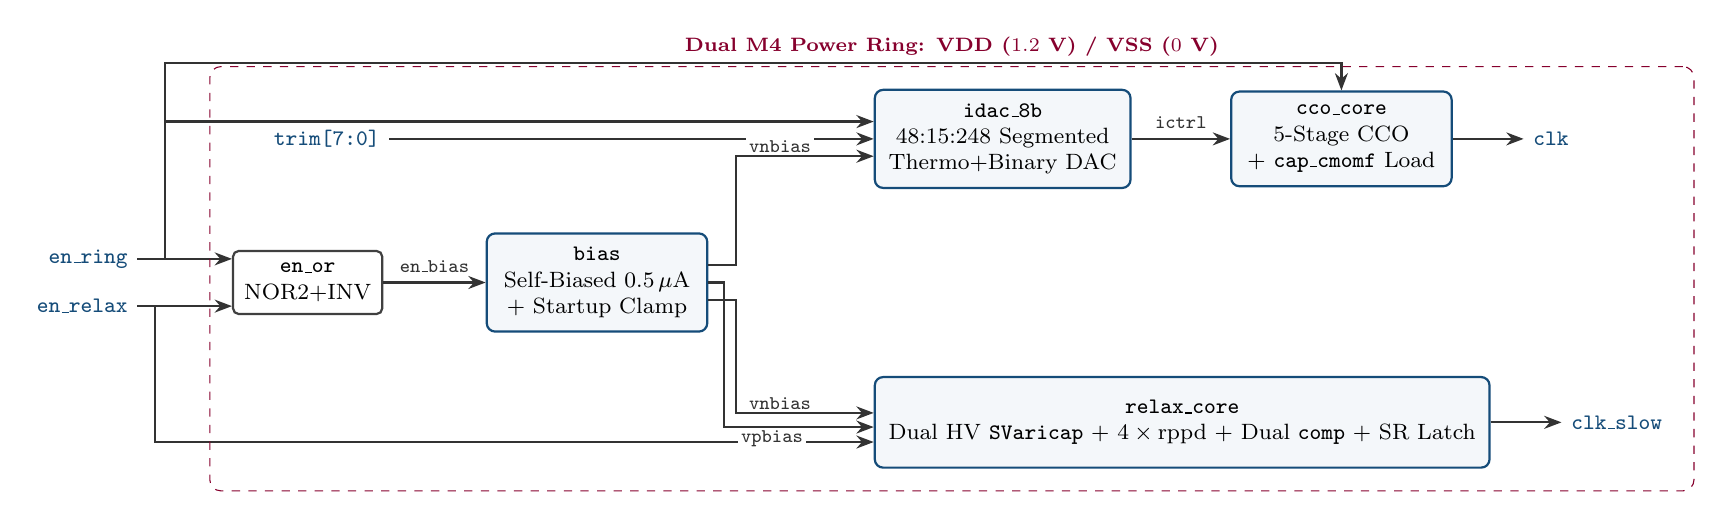
\begin{tikzpicture}[
  font=\footnotesize,
  blk/.style={draw=AccentBlue, thick, fill=SoftBg, rounded corners=3pt, minimum height=1.15cm, align=center, inner sep=5pt},
  gate/.style={draw=black!75, thick, fill=white, rounded corners=2pt, minimum height=0.8cm, align=center, inner sep=4pt},
  arr/.style={-{Stealth[length=2.2mm]}, thick, color=black!80},
  io/.style={font=\ttfamily\footnotesize\bfseries, color=AccentBlue}
]
  \node[gate] (enor) {\texttt{en\_or}\\NOR2+INV};
  \node[blk, right=1.3cm of enor, minimum width=2.8cm] (bias) {\textbf{\texttt{bias}}\\Self-Biased $0.5\,\mu\text{A}$\\+ Startup Clamp};
  \node[blk, above right=0.55cm and 2.1cm of bias, minimum width=2.9cm] (idac) {\textbf{\texttt{idac\_8b}}\\48:15:248 Segmented\\Thermo+Binary DAC};
  \node[blk, right=1.25cm of idac, minimum width=2.8cm] (cco) {\textbf{\texttt{cco\_core}}\\5-Stage CCO\\+ \texttt{cap\_cmomf} Load};
  \node[blk, below right=0.55cm and 2.1cm of bias, minimum width=5.6cm] (relax) {\textbf{\texttt{relax\_core}}\\Dual HV \texttt{SVaricap} + $4\times\text{rppd}$ + Dual \texttt{comp} + SR Latch};

  % West Inputs
  \node[io, left=1.2cm of enor, yshift=3mm] (in_ring) {en\_ring};
  \node[io, left=1.2cm of enor, yshift=-3mm] (in_rel) {en\_relax};
  \node[io, left=6.15cm of idac] (in_trim) {trim[7:0]};

  \draw[arr] (in_ring) -- (enor.west |- in_ring);
  \draw[arr] (in_rel) -- (enor.west |- in_rel);
  \draw[arr] (in_ring.east) -- ++(0.35,0) |- ($(idac.west)+(0,0.22)$);
  \draw[arr] (in_ring.east) -- ++(0.35,0) |- ($(cco.north)+(0,0.35)$) -- (cco.north);
  \draw[arr] (in_rel.east) -- ++(0.22,0) |- ($(relax.west)+(0,-0.25)$);
  \draw[arr] (in_trim) -- (idac.west);

  \draw[arr] (enor) -- node[above, font=\scriptsize\ttfamily]{en\_bias} (bias);
  \draw[arr] ($(bias.east)+(0,0.22)$) -- ++(0.35,0) |- node[pos=0.66, above, font=\scriptsize\ttfamily, fill=white, inner sep=1pt]{vnbias} ($(idac.west)+(0,-0.22)$);
  \draw[arr] ($(bias.east)+(0,-0.22)$) -- ++(0.35,0) |- node[pos=0.66, above, font=\scriptsize\ttfamily, fill=white, inner sep=1pt]{vnbias} ($(relax.west)+(0,0.12)$);
  \draw[arr] ($(bias.east)+(0,0.0)$) -- ++(0.20,0) |- node[pos=0.66, below, font=\scriptsize\ttfamily, fill=white, inner sep=1pt]{vpbias} ($(relax.west)+(0,-0.06)$);

  \draw[arr] (idac) -- node[above, font=\scriptsize\ttfamily]{ictrl} (cco);

  % East Outputs
  \node[io, right=0.9cm of cco] (out_clk) {clk};
  \node[io, right=0.9cm of relax] (out_slow) {clk\_slow};
  \draw[arr] (cco) -- (out_clk);
  \draw[arr] (relax) -- (out_slow);

  % Power Ring Note
  \node[draw=purple!70!black, dashed, rounded corners=4pt, fit=(enor)(bias)(idac)(cco)(relax)(out_slow), inner sep=8pt, label={[font=\scriptsize\bfseries, color=purple!70!black]above:Dual M4 Power Ring: VDD ($1.2\text{ V}$) / VSS ($0\text{ V}$)}] {};
\end{tikzpicture}%
}
\caption{Block diagram of the unified \texttt{rpe\_clk\_analog} macro showing shared bias distribution and independent enable gating.}
\label{fig:macro_arch}
\end{figure}

\subsection{High-Speed Ring Oscillator Selection (Ring A vs.\ Ring B)}
Two complete ring-oscillator topologies were designed and simulated across PVT before committing to silicon layout: \textbf{Ring A} (\texttt{osc\_ring\_std}), an unregulated current-starved standard-cell chain using an 8-bit NMOS binary tail array, and \textbf{Ring B} (\texttt{osc\_ring\_cc}), a current-controlled 5-stage ring loaded by MOM capacitors (\texttt{cap\_cmomf}) and driven by a segmented PMOS current DAC (\texttt{idac\_8b}) referenced to \texttt{bias}. After post-layout PEX quantification (Sec.~\ref{sec:pex}), Ring B was co-centered for layout parasitics ($2.4\times 2.4\,\mu\text{m}$ CMOMF load + $1.33\times$ master drive boost), elevating schematic mid-range frequency while centering Magic PEX at \texttt{trim=155}. Table~\ref{tab:ring_tradeoff} compares Ring A (schematic) against the final PEX-centered Ring B.

\begin{table}[H]
\centering
\caption{Trade-Off Matrix: Standard Starved Ring (Ring A) vs.\ Current-Controlled CMOM Ring (Ring B).}
\label{tab:ring_tradeoff}
\footnotesize
\setlength{\tabcolsep}{4pt}
\begin{tabularx}{\textwidth}{@{}>{\raggedright\arraybackslash}p{3.4cm} >{\raggedright\arraybackslash}X >{\raggedright\arraybackslash}X >{\raggedright\arraybackslash}p{3.1cm}@{}}
\toprule
\textbf{Metric} & \textbf{Ring A (\texttt{osc\_ring\_std}, Sch.)} & \textbf{Ring B (\texttt{osc\_ring\_cc}, Sch.\ / PEX)} & \textbf{Decision Impact} \\
\midrule
Tuning Range (\texttt{tt}, $1.20\text{ V}$, $25\,^\circ\text{C}$) & $23.80$--$130.20\text{ MHz}$ & $35.14$--$193.63$ (Sch.) / $15.84$--$83.77\text{ MHz}$ (PEX) & Covers $60\text{ MHz}$ post-PEX \\
Boot \texttt{trim=128} (\texttt{tt}/\texttt{ss}/\texttt{ff}) & $40.36 / 25.07 / \mathbf{61.28}\text{ MHz}$ & PEX: $52.78 / 52.98 / \mathbf{58.51}\text{ MHz}$ & \textbf{Ring B $\le 60\text{ MHz}$ in \texttt{ff}} \\
Nominal $60\text{ MHz}$ Point & \texttt{trim=191}: $61.28\text{ MHz}$, $86.3\,\mu\text{A}$ & \texttt{trim=38} Sch.\ ($61.60\text{ MHz}$) / \texttt{155} PEX ($59.92\text{ MHz}$, $61.5\,\mu\text{A}$) & Ring B saves $29\%$ current \\
Duty Cycle @ $\sim 60\text{ MHz}$ (\texttt{tt}) & $51.93\%$ & $50.51\%$ (Sch.\ @ 38) / $48.74\%$ (PEX @ 155) & Near-ideal $50\%$ symmetry \\
Supply Sensitivity ($1.08$--$1.32\text{ V}$) & $+161.5\%/\text{V}$ ($49.33 \to 73.08\text{ MHz}$) & $-45.0\%/\text{V}$ ($64.43 \to 57.77\text{ MHz}$ @ \texttt{38}) & \textbf{$3.6\times$ lower VDD sens.} \\
Temp.\ Drift ($-40$--$125\,^\circ\text{C}$) & $-13.6\%$ ($64.80 \to 56.45\text{ MHz}$) & $+53.1\%$ ($49.96 \to 82.67\text{ MHz}$ @ \texttt{38}) & PTAT \texttt{bias} dominates Ring B \\
Tuning Linearity & Exponential ($0.55\text{ MHz}$ @ 191) & Linear ($\sim 0.43\%/\text{LSB}$ @ PEX 155) & Uniform trim slope \\
Binary 127$\to$128 Step & $40.353 \to 40.351\text{ MHz}$ & $120.484 \to 121.028\text{ MHz}$ (thermo, Sch.) & $48{:}15{:}248$ avoids glitches \\
\bottomrule
\end{tabularx}
\end{table}

Ring B was selected because an unregulated CMOS ring in \texttt{ff} ($1.32\text{ V}$, $-40\,^\circ\text{C}$) exceeds the $60\text{ MHz}$ SoC digital timing ceiling at its default mid-scale boot trim ($61.28\text{ MHz}$ at \texttt{trim=128}), and its $+161.5\%/\text{V}$ supply slope leaves it vulnerable to SoC IR drop. With parasitic pre-emphasis, Ring B clusters tightly across \texttt{tt}/\texttt{ss}/\texttt{ff} at boot \texttt{trim=128} post-layout ($52.78 / 52.98 / 58.51\text{ MHz}$ in Magic PEX), consumes $29\%$ less current than Ring A at $60\text{ MHz}$, and yields a linear $0.43\%/\text{LSB}$ transfer curve.

\subsection{Relaxation Oscillator Architecture Trade-Off (4 Options)}
A $100\text{ kHz}$ RC relaxation oscillator using nanoampere charging currents faces a severe area--leakage trade-off in $130\text{ nm}$ CMOS. We evaluated four physical implementations mixing capacitor type (\texttt{cap\_cmomf} MIM/MOM stack vs.\ $3.3\text{ V}$ \texttt{SVaricap} thick-gate-oxide MOSCAP) and mirror current scaling ($M=10$ yielding $\sim 50\text{ nA}$ vs.\ $M=1$ yielding $\sim 500\text{ nA}$), using identical dual-slope architecture and $4\times\text{rppd}$ poly resistors ($\approx 1{,}800\,\mu\text{m}^2$).

\begin{table}[H]
\centering
\caption{Relaxation Oscillator Architecture Comparison (\texttt{osc\_relax\_options.csv}).}
\label{tab:relax_tradeoff}
\footnotesize
\setlength{\tabcolsep}{4pt}
\begin{tabularx}{\textwidth}{@{}llcccc >{\raggedright\arraybackslash}X@{}}
\toprule
\textbf{Option} & \textbf{$M$ ($I_{\text{chg}}$)} & \textbf{Freq (\texttt{tt})} & \textbf{VDD Sens.} & \textbf{Temp Drift} & \textbf{125\,$^\circ$C Leak} & \textbf{Est.\ Passive Area} \\
\midrule
\texttt{cmomf\_M10} & $10$ ($\sim 50\text{ nA}$) & $111.12\text{ kHz}$ & $+12.00\%/\text{V}$ & $-4.99\%$ & $0.000\text{ nA}$ & $\sim 2{,}730\,\mu\text{m}^2$ ($1800\text{R}+930\text{C}$) \\
\texttt{cmomf\_M1} & $1$ ($\sim 500\text{ nA}$) & $110.87\text{ kHz}$ & $+14.56\%/\text{V}$ & $-5.52\%$ & $0.000\text{ nA}$ & $\sim 11{,}100\,\mu\text{m}^2$ ($1800\text{R}+9300\text{C}$) \\
\rowcolor{PassBg} \textbf{\texttt{hv\_moscap\_M10}} & $\mathbf{10}$ ($\mathbf{\sim 50\text{ nA}}$) & $\mathbf{97.24}\text{ kHz}^*$ & $\mathbf{+9.99\%/\text{V}}$ & $\mathbf{-4.92\%}$ & $\mathbf{0.000\text{ nA}}$ & $\mathbf{\sim 2{,}050\,\mu\text{m}^2}$ ($1800\text{R}+250\text{C}$) \\
\texttt{hv\_moscap\_M1} & $1$ ($\sim 500\text{ nA}$) & $96.30\text{ kHz}$ & $+12.51\%/\text{V}$ & $-3.98\%$ & $0.000\text{ nA}$ & $\sim 4{,}300\,\mu\text{m}^2$ ($1800\text{R}+2500\text{C}$) \\
\bottomrule
\end{tabularx}
\begin{flushleft}\footnotesize $^*$In \texttt{relax\_core}, \texttt{SVaricap} fingers were tuned from $N_x=9$ to $N_x=8$ ($w=9.74\,\mu\text{m}, l=0.8\,\mu\text{m}$) so post-layout PEX centers \texttt{sleep\_relax} at $98.54\text{ kHz}$ ($112.07\text{ kHz}$ schematic; Table~\ref{tab:pex_vs_sch}).\end{flushleft}
\end{table}

\textbf{\texttt{hv\_moscap\_M10}} was selected: thin-oxide $1.2\text{ V}$ MOSCAPs would leak severely against $50\text{ nA}$, whereas $3.3\text{ V}$ \texttt{SVaricap} exhibits $0.0000\text{ nA}$ simulated gate leakage even at $125\,^\circ\text{C}$ alongside higher capacitance density ($C_{\text{ox}}$ of thick oxide $\approx 4\times$ dense as \texttt{cap\_cmomf}). Combined with $M=10$ current division and \texttt{nmosHV} ($3.3\text{ V}$) discharge switches ($0.0004\text{ nA}$ switch leakage at $125\,^\circ\text{C}$), the integrated capacitor bank shrinks from $9{,}300\,\mu\text{m}^2$ to $\sim 250\,\mu\text{m}^2$ and achieves the lowest supply sensitivity ($+9.99\%/\text{V}$).

% =============================================================================
% SECTION 2: PDK & METHODOLOGY
% =============================================================================
\section{Process Technology, PDK \& Verification Methodology}

All circuits target IHP's open-source \texttt{ihp-sg13cmos5l} $130\text{ nm}$ CMOS5L stack ($4$ thin aluminum routing metals \texttt{Metal1}--\texttt{Metal4} plus thicker top metals disabled here by \texttt{CMOS5L.FORB} rules). Core logic and analog devices use \texttt{sg13\_lv\_nmos} / \texttt{sg13\_lv\_pmos} ($1.2\text{ V}$) and standard cells from \texttt{sg13cmos5l\_stdcell}. High-threshold, ultra-low-leakage nodes inside \texttt{relax\_core} utilize \texttt{SG13\_dev} thick-gate-oxide (\texttt{TGO}) primitives \texttt{sg13\_hv\_nmos} (\texttt{nmosHV}) and \texttt{sg13\_hv\_svaricap} (\texttt{SVaricap}), while precision resistors use unsalicided polysilicon (\texttt{rppd}) with \texttt{SalBlock}.

Schematics were drawn and netlisted in \texttt{xschem} and simulated in \texttt{ngspice} across three extremal corners: \texttt{tt} ($1.20\text{ V}$, $25\,^\circ\text{C}$), \texttt{ss} ($1.08\text{ V}$, $125\,^\circ\text{C}$), and \texttt{ff} ($1.32\text{ V}$, $-40\,^\circ\text{C}$), using a uniform initial-condition transient harness (\texttt{.tran 5n 44u uic}) for multi-mode macro verification. Custom layouts were synthesized programmatically in Python using KLayout 0.30.12 and native IHP \texttt{SG13\_dev} PCells, then checked against the full PDK \texttt{ihp-sg13cmos5l.drc} (\texttt{tables=main} and \texttt{tables="main antenna"}) and \texttt{sg13cmos5l.lvs} runsets in strict port mode.

% =============================================================================
% SECTION 3: CIRCUIT DESIGN & SIMULATION
% =============================================================================
\section{Circuit Design \& Simulation Characterization}

\subsection{Shared Self-Biased Startup Reference (\texttt{bias})}
The \texttt{bias} cell (Figure~\ref{fig:sch_bias}) implements a beta-multiplier self-biased reference around \texttt{R\_BIAS} (\texttt{rppd}, $w=0.5\,\mu\text{m}$, $l=20.0\,\mu\text{m}$, $b=19$, $\approx 108\text{ k}\Omega$) with $4{:}1$ NMOS aspect ratio (\texttt{MN2} $m=4$ vs.\ \texttt{MN1} $m=1$, $0.3\,\mu\text{m}/4.0\,\mu\text{m}$) and cascode-length ($4.0\,\mu\text{m}$) PMOS mirrors. A zero-DC-current startup chain (\texttt{MSU\_EN}, two $0.15\,\mu\text{m}/10\,\mu\text{m}$ weak PMOS \texttt{MSU\_P1/P2}, sense NMOS \texttt{MSU\_N}, and injection transistor \texttt{MSU\_INJ}) nudges \texttt{vpbias} low upon power-up and turns off automatically once \texttt{vnbias} settles. When \texttt{en=0}, \texttt{MP\_OFF} and \texttt{MN\_OFF} clamp \texttt{vpbias}$\to V_{DD}$ and \texttt{vnbias}$\to V_{SS}$.

\begin{figure}[H]
\centering
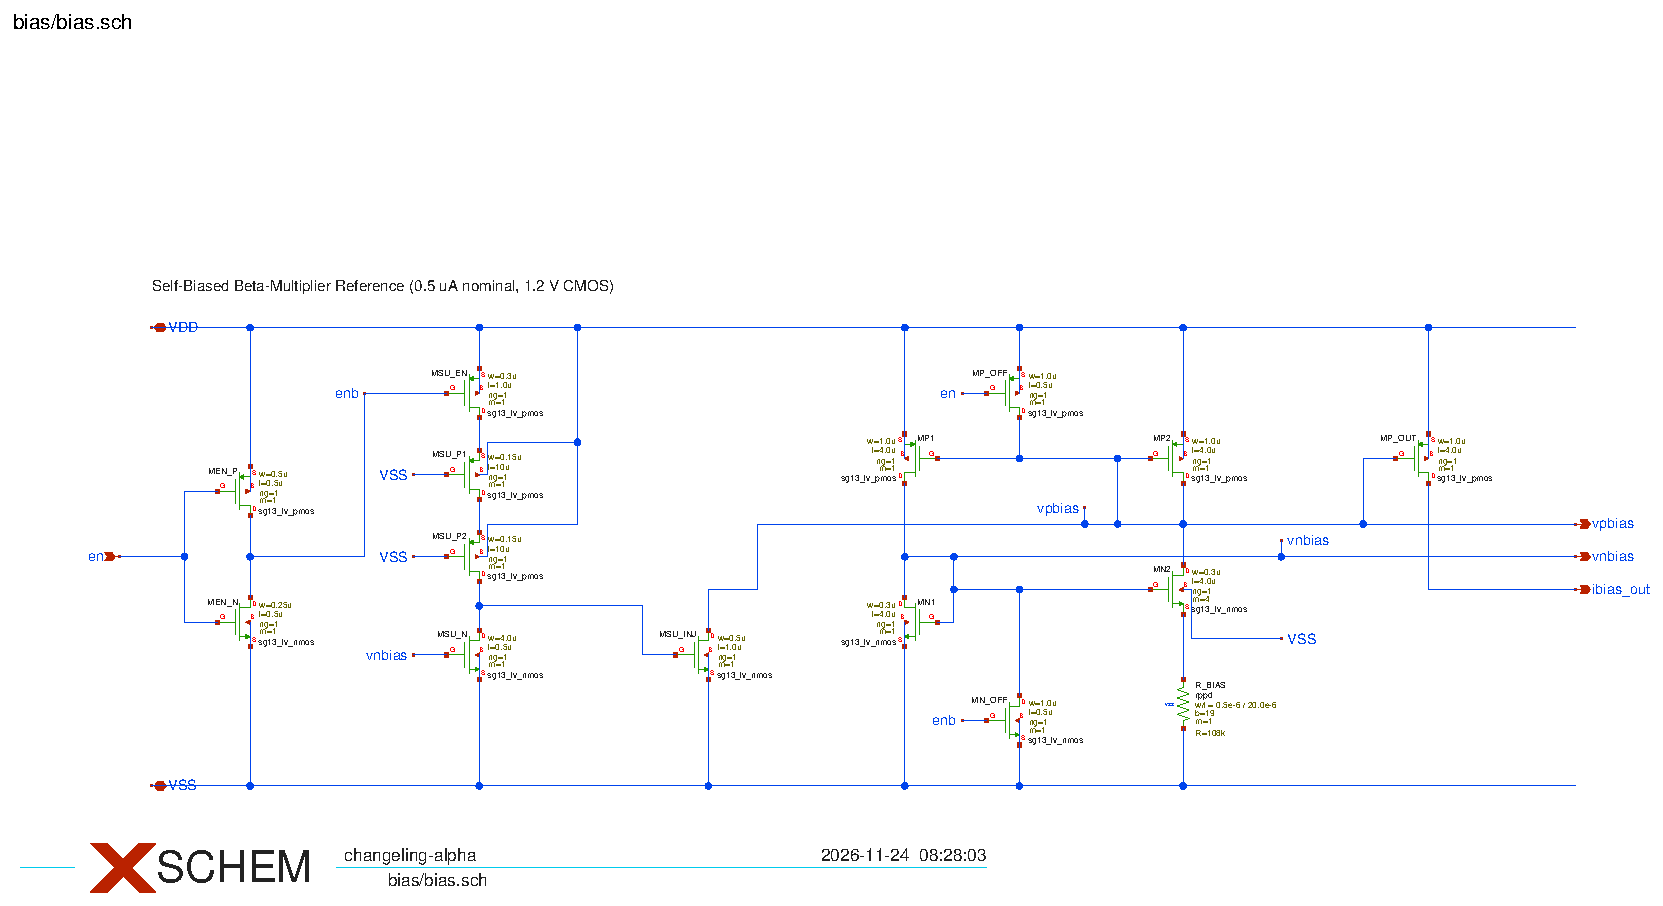
\includegraphics[width=0.92\textwidth]{figures/sch_bias.pdf}
\caption{Schematic of the shared $0.5\,\mu\text{A}$ self-biased reference and startup circuit (\texttt{bias}).}
\label{fig:sch_bias}
\end{figure}

Figure~\ref{fig:bias_pvt} and Table~\ref{tab:bias_corners} summarize PVT regulation, PTAT behavior ($\Delta V_{GS}/R$ increases with temperature while negative-TC poly resistance reinforces the positive slope), and sub-$8.5\,\mu\text{s}$ deterministic startup across corners.

\begin{figure}[H]
\centering
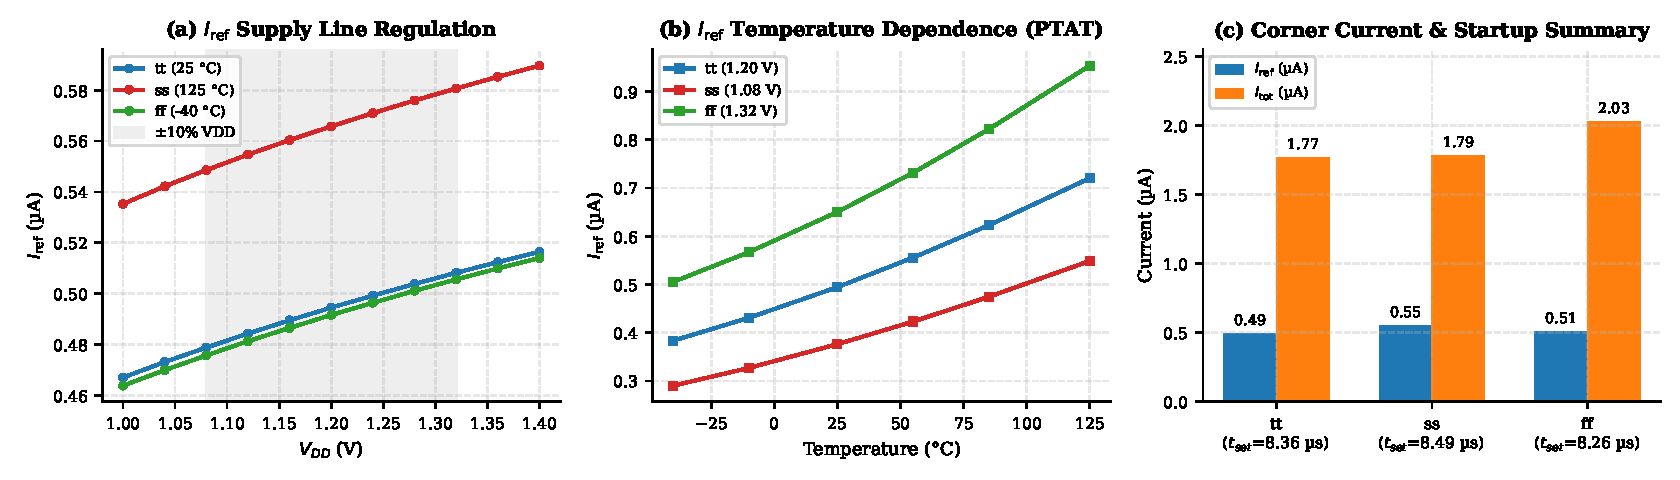
\includegraphics[width=\textwidth]{figures/fig_bias_pvt.pdf}
\caption{Bias reference PVT characterization: (a) $I_{\text{ref}}$ line regulation, (b) temperature sweep ($-40$ to $125\,^\circ\text{C}$), and (c) corner summary with startup settling time.}
\label{fig:bias_pvt}
\end{figure}

\begin{table}[H]
\centering
\caption{Verified \texttt{bias} Corner \& Startup Summary (\texttt{bias\_corners.csv}, \texttt{bias\_startup.csv}).}
\label{tab:bias_corners}
\small
\begin{tabular}{@{}ccccccccc@{}}
\toprule
\textbf{Corner} & \textbf{$V_{DD}$ (V)} & \textbf{Temp ($^\circ\text{C}$)} & \textbf{$I_{\text{ref}}$ ($\mu\text{A}$)} & \textbf{$I_{\text{tot}}$ ($\mu\text{A}$)} & \textbf{$V_{\text{pbias}}$ (V)} & \textbf{$V_{\text{nbias}}$ (V)} & \textbf{$I_{\text{standby}}$ (nA)} & \textbf{$t_{\text{settle}}$ ($\mu\text{s}$)} \\
\midrule
\texttt{tt} & $1.20$ & $25$ & $0.4945$ & $1.7672$ & $0.6580$ & $0.4067$ & $0.7164$ & $8.356$ \\
\texttt{ss} & $1.08$ & $125$ & $0.5486$ & $1.7858$ & $0.5023$ & $0.4603$ & $4.5509$ & $8.494$ \\
\texttt{ff} & $1.32$ & $-40$ & $0.5056$ & $2.0303$ & $0.8215$ & $0.3645$ & $1.2610$ & $8.264$ \\
\bottomrule
\end{tabular}
\end{table}

\subsection{Current-Controlled Ring Oscillator (\texttt{idac\_8b} + \texttt{cco\_core})}
The 8-bit current DAC (\texttt{idac\_8b}, Figure~\ref{fig:sch_idac}) mirrors \texttt{vnbias} into a diode-connected PMOS master (\texttt{MP\_IN}, $m=2$, $1.5/4.0\,\mu\text{m}$, giving $1.33\times$ current gain vs.\ $2.0\,\mu\text{m}$ to pre-compensate layout parasitics) feeding $48$ pedestal units (\texttt{PED}), $1{:}2{:}4{:}8{:}16$ binary LSB units (\texttt{B0}--\texttt{B4}, \texttt{trim[4:0]}), and $7 \times 32 = 224$ thermometer MSB units (\texttt{T0}--\texttt{T6}, decoded from \texttt{trim[7:5]} by $18$ standard cells). This $48{:}15{:}248$ segmentation ensures monotonic switching and positive pedestal current at \texttt{trim=0}. The summed \texttt{ictrl} current is mirrored into symmetric NMOS/PMOS current-starving headers across $5$ stages in \texttt{cco\_core} (Figure~\ref{fig:sch_cco}), each loaded by a downsized $2.4 \times 2.4\,\mu\text{m}$ \texttt{cap\_cmomf} ($7.41\text{ fF}$ compact / $\approx 10\text{ fF}$ extracted) and buffered by \texttt{XBUF1/2/4} (\texttt{inv\_1}$\to$\texttt{inv\_2}$\to$\texttt{buf\_4}).

\begin{figure}[H]
\centering
\begin{minipage}[b]{0.51\textwidth}
  \centering
  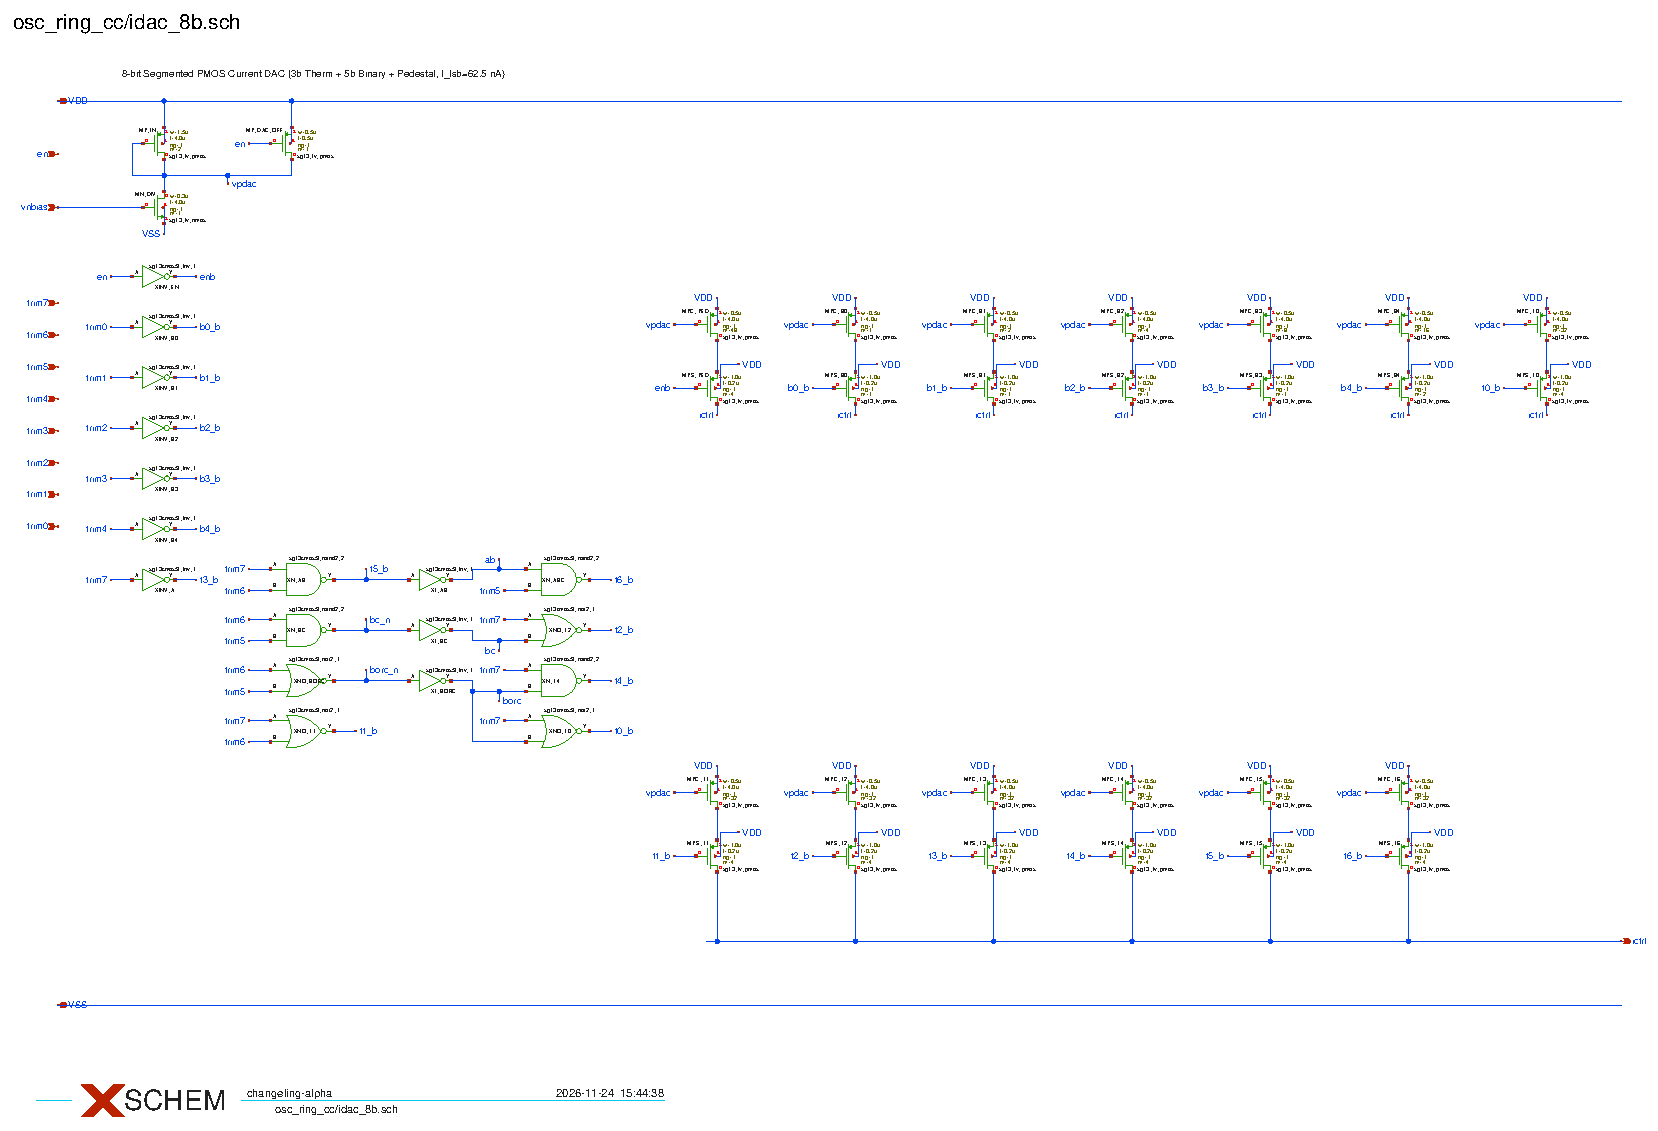
\includegraphics[width=\textwidth]{figures/sch_idac_8b.pdf}
  \caption{8-bit segmented \texttt{idac\_8b} schematic.}
  \label{fig:sch_idac}
\end{minipage}\hfill
\begin{minipage}[b]{0.47\textwidth}
  \centering
  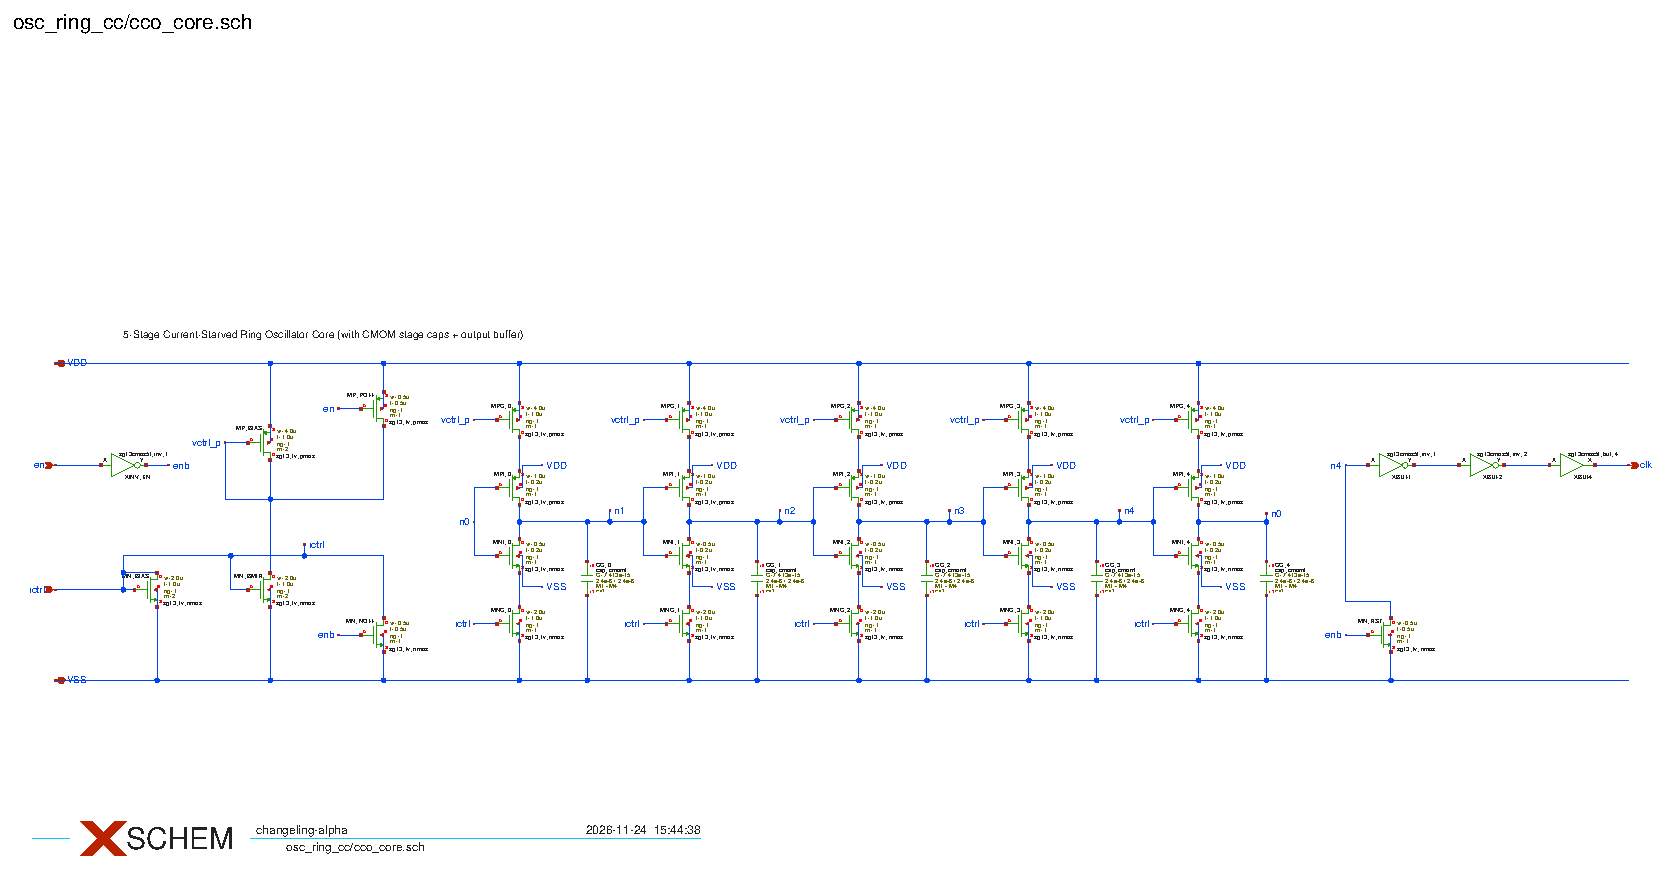
\includegraphics[width=\textwidth]{figures/sch_cco_core.pdf}
  \caption{5-stage CMOM-loaded \texttt{cco\_core} schematic.}
  \label{fig:sch_cco}
\end{minipage}
\end{figure}

Figure~\ref{fig:ring_trim} contrasts the tuning behavior of Ring A vs.\ Ring B across PVT, while Figure~\ref{fig:ring_sensitivity} shows supply and temperature sensitivity plus the verified $1.20 \to 1.25\text{ V}$ supply step response of Ring B at \texttt{trim=38} ($61.59 \to 59.30 \to 59.99\text{ MHz}$). Note that Ring B exhibits a $+53.1\%$ schematic frequency rise from $-40$ to $125\,^\circ\text{C}$ because the shared PTAT \texttt{bias} current nearly doubles over temperature ($0.3838$ to $0.7200\,\mu\text{A}$); at extremal fast/cold (\texttt{ff}) and slow/hot (\texttt{ss}) corners, higher \texttt{ss} bias current compensates slower MOSFETs, keeping the three PVT curves closely aligned ($39.55$--$179.22\text{ MHz}$ \texttt{ss}, $36.47$--$218.57\text{ MHz}$ \texttt{ff} pre-PEX; $17.32$--$78.08\text{ MHz}$ \texttt{ss}, $16.99$--$96.89\text{ MHz}$ \texttt{ff} post-PEX).

\begin{figure}[H]
\centering
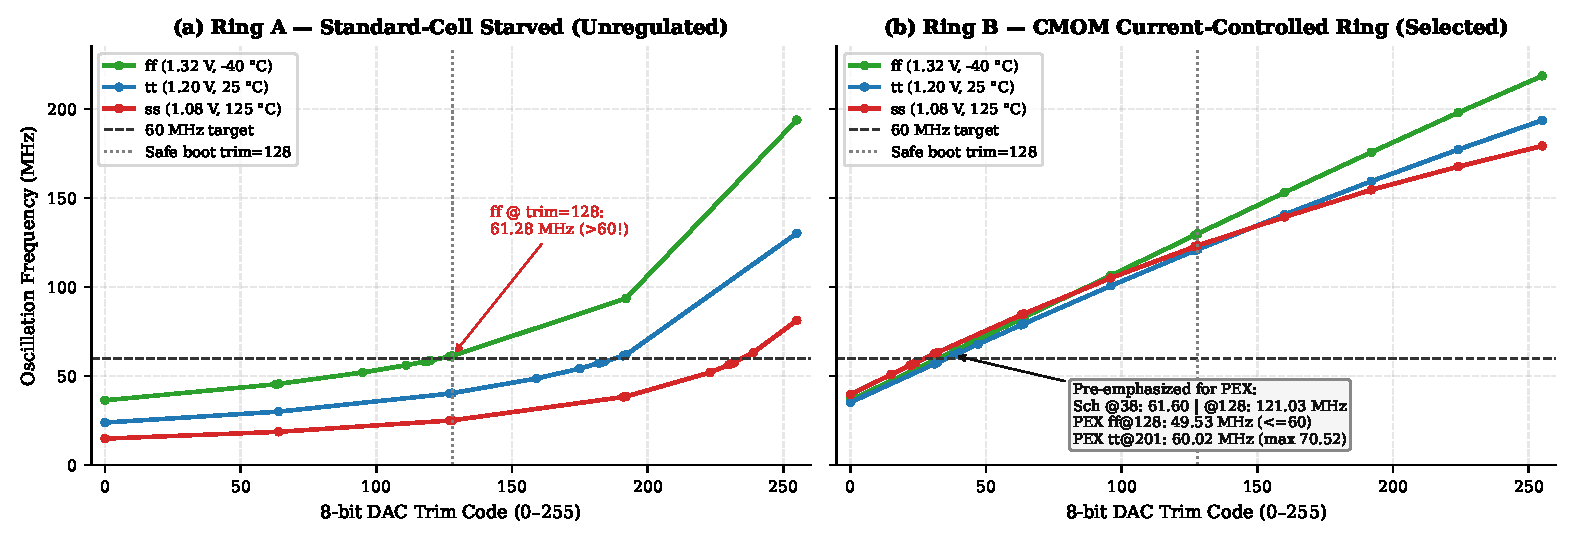
\includegraphics[width=\textwidth]{figures/fig_ring_trim.pdf}
\caption{Tuning characteristics across \texttt{tt}/\texttt{ss}/\texttt{ff}: (a) Ring A exceeds $60\text{ MHz}$ in \texttt{ff} at \texttt{trim=128}; (b) Ring B schematic is pre-emphasized for layout parasitics so Magic PEX hits $59.92\text{ MHz}$ (\texttt{tt}, \texttt{trim=155}) while staying $\le 60\text{ MHz}$ at boot (\texttt{trim=128}).}
\label{fig:ring_trim}
\end{figure}

\begin{figure}[H]
\centering
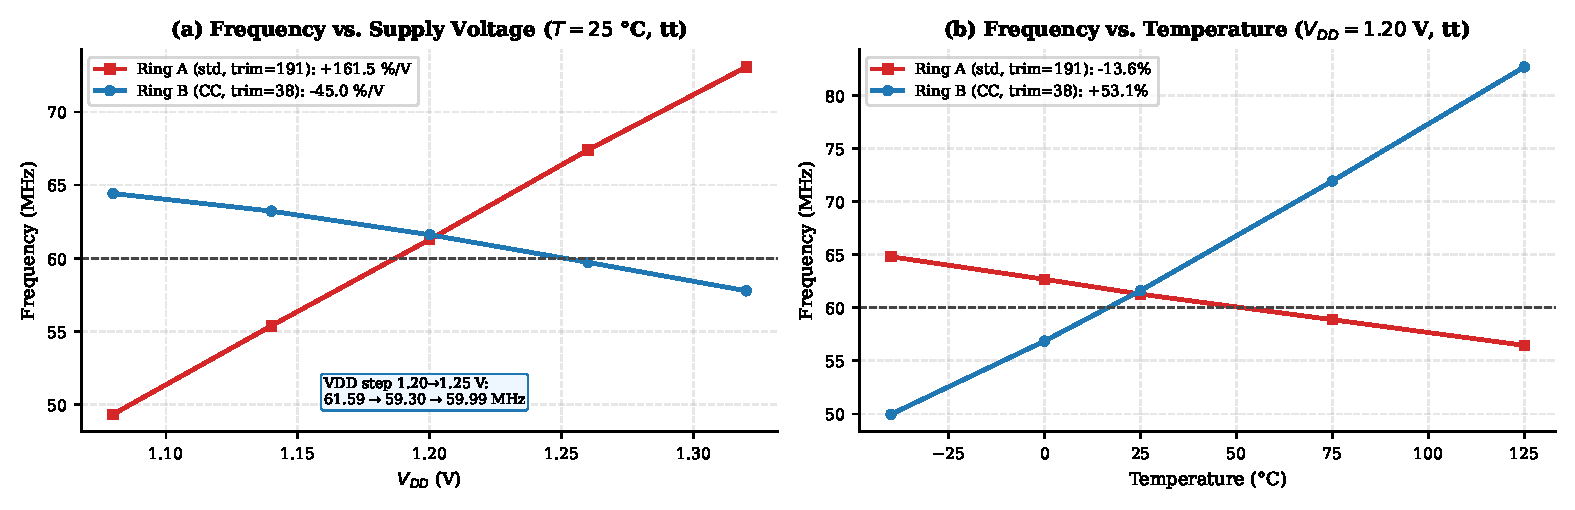
\includegraphics[width=\textwidth]{figures/fig_ring_sensitivity.pdf}
\caption{Ring A vs.\ Ring B environmental sensitivity: (a) $V_{DD}$ sweep ($-45.0\%/\text{V}$ vs.\ $+161.5\%/\text{V}$) with Ring B $1.20 \to 1.25\text{ V}$ step annotation; (b) temperature sweep.}
\label{fig:ring_sensitivity}
\end{figure}

\subsection{Dual-Slope HV Relaxation Oscillator (\texttt{relax\_core} + \texttt{comp})}
In \texttt{relax\_core} (Figure~\ref{fig:sch_relax}), \texttt{MP\_REF} mirrors \texttt{bias} current ($\sim 0.49\,\mu\text{A}$) through four series \texttt{rppd} segments ($4 \times 40\,\mu\text{m}/0.5\,\mu\text{m}$, $b=9$, total $\approx 836\text{ k}\Omega$) to establish a supply-insensitive threshold $V_{\text{th}} \approx 0.415\text{ V}$. A $10{:}1$ PMOS divider (\texttt{MP\_CHG\_IN} $m=10$) supplies $\approx 50\text{ nA}$ alternately to two $8$-finger HV \texttt{SVaricap} integrators (\texttt{C\_A}, \texttt{C\_B}, $w=9.74\,\mu\text{m}, l=0.8\,\mu\text{m}$, reduced from $N_x=9$ to absorb routing and comparator capacitance) monitored by two continuous-time 2-stage comparators (\texttt{comp}, Figure~\ref{fig:sch_comp}). Cross-coupled \texttt{NOR} gates alternate which tank integrates while \texttt{nmosHV} pull-downs (\texttt{MN\_DIS\_A/B}) hold the idle tank discharged; an anti-deadlock \texttt{NAND} (\texttt{XBOTH\_NAND}$\to$\texttt{MN\_UNSTICK}) guarantees oscillation recovery if both tanks exceed $V_{\text{th}}$ simultaneously.

\begin{figure}[H]
\centering
\begin{minipage}[b]{0.55\textwidth}
  \centering
  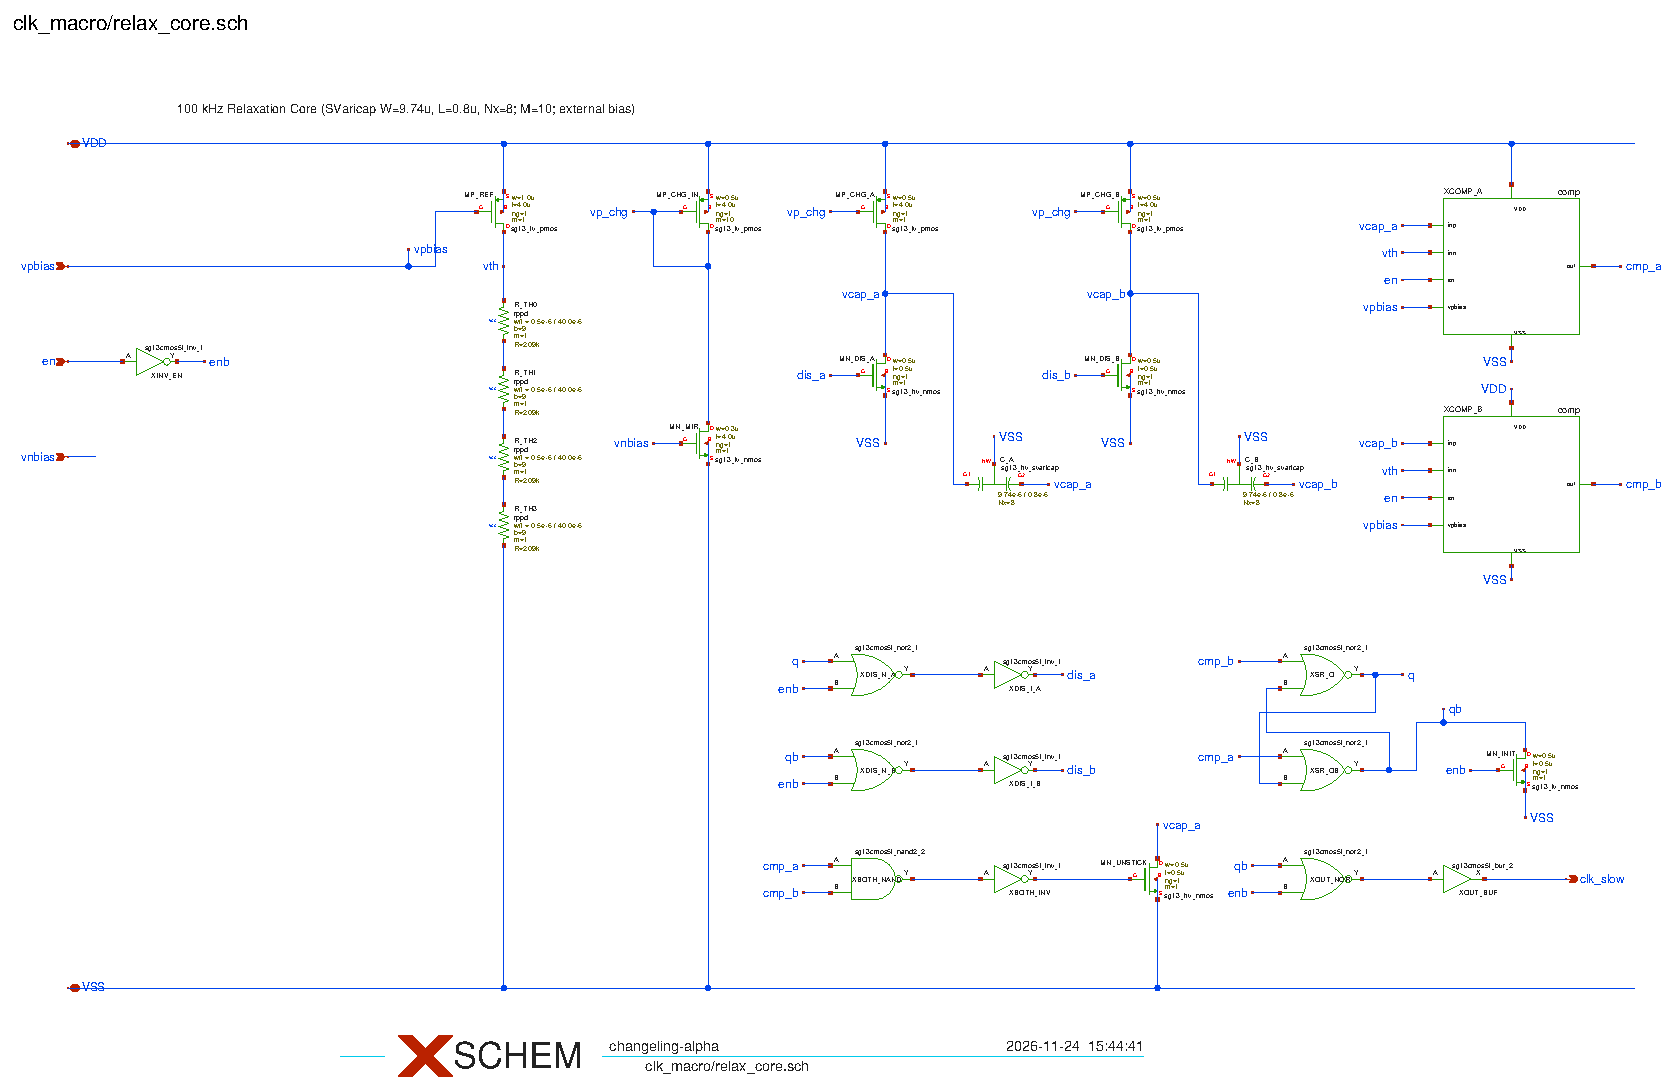
\includegraphics[width=\textwidth]{figures/sch_relax_core.pdf}
  \caption{\texttt{relax\_core} dual-slope schematic.}
  \label{fig:sch_relax}
\end{minipage}\hfill
\begin{minipage}[b]{0.43\textwidth}
  \centering
  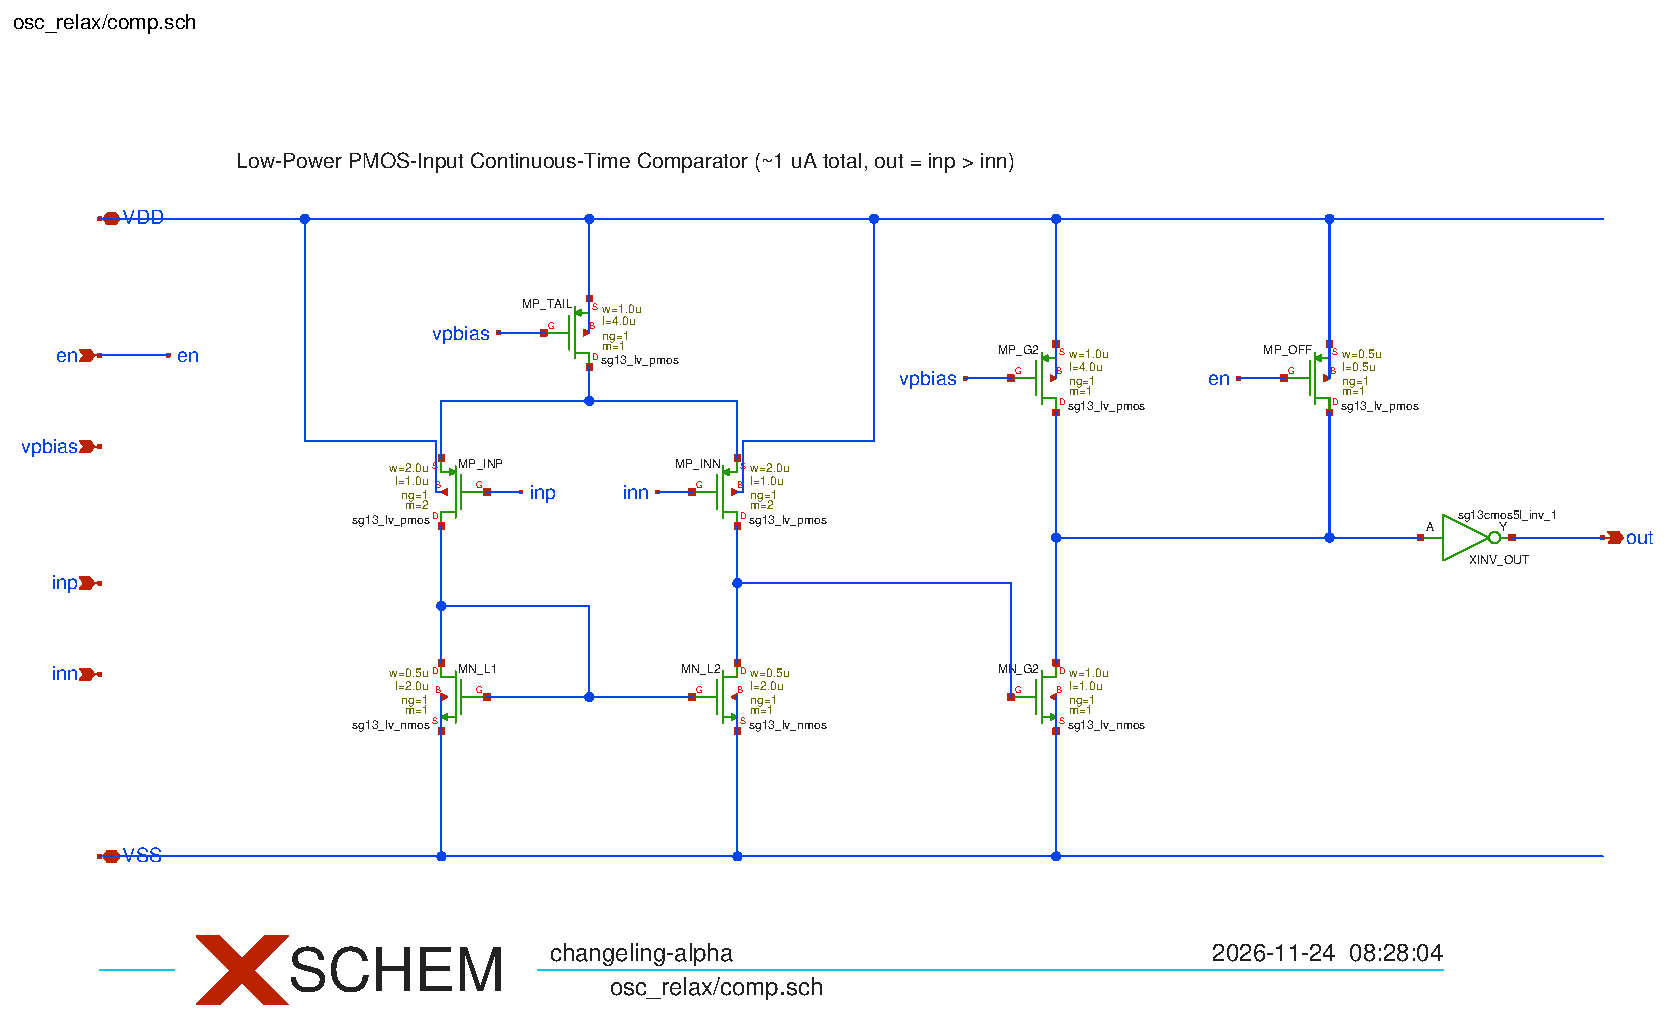
\includegraphics[width=\textwidth]{figures/sch_comp.pdf}
  \caption{2-stage comparator (\texttt{comp}) schematic.}
  \label{fig:sch_comp}
\end{minipage}
\end{figure}

Figure~\ref{fig:relax_options} summarizes passive area vs.\ supply sensitivity across all four candidates alongside the temperature and supply drift curves for the \texttt{cmomf\_M10} sweep ($109.56$--$112.76\text{ kHz}$ over $V_{DD}$, $113.02$--$107.47\text{ kHz}$ over temperature, with \texttt{hv\_moscap\_M10} achieving even tighter $+9.99\%/\text{V}$ supply regulation).

\begin{figure}[H]
\centering
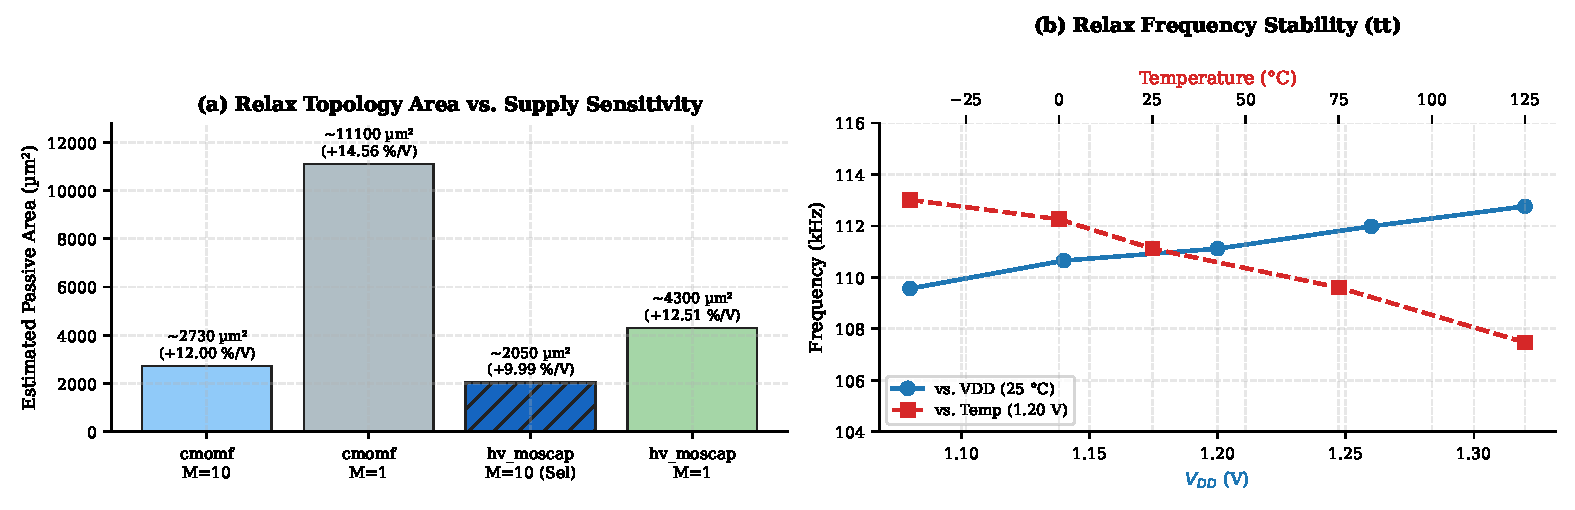
\includegraphics[width=\textwidth]{figures/fig_relax_options.pdf}
\caption{(a) Comparison of estimated passive area and supply sensitivity across the four relaxation oscillator topologies; (b) supply and temperature stability curves (\texttt{tt}).}
\label{fig:relax_options}
\end{figure}

\subsection{Unified \texttt{rpe\_clk\_analog} Top-Level Multi-Mode Verification}
The integrated macro testbench (\texttt{rpe\_clk\_analog}, Figure~\ref{fig:sch_top}) was verified in both schematic and Magic PEX netlists across all five operating states (\texttt{standby}, \texttt{ring\_only trim=128}, \texttt{ring\_only trim=155}, \texttt{sleep\_relax}, and \texttt{both\_active trim=155}) and all three corners (\texttt{tt}/\texttt{ss}/\texttt{ff}). Table~\ref{tab:macro_modes} reports the pre-layout schematic baseline measurements from \texttt{clk\_macro\_modes.csv} (reflecting intentional capacitive/drive pre-emphasis; post-layout PEX results follow in Table~\ref{tab:pex_vs_sch}), and Figure~\ref{fig:macro_wf} plots internal CCO stage and dual-slope relaxation waveforms from the unified schematic runs.

\begin{figure}[H]
\centering
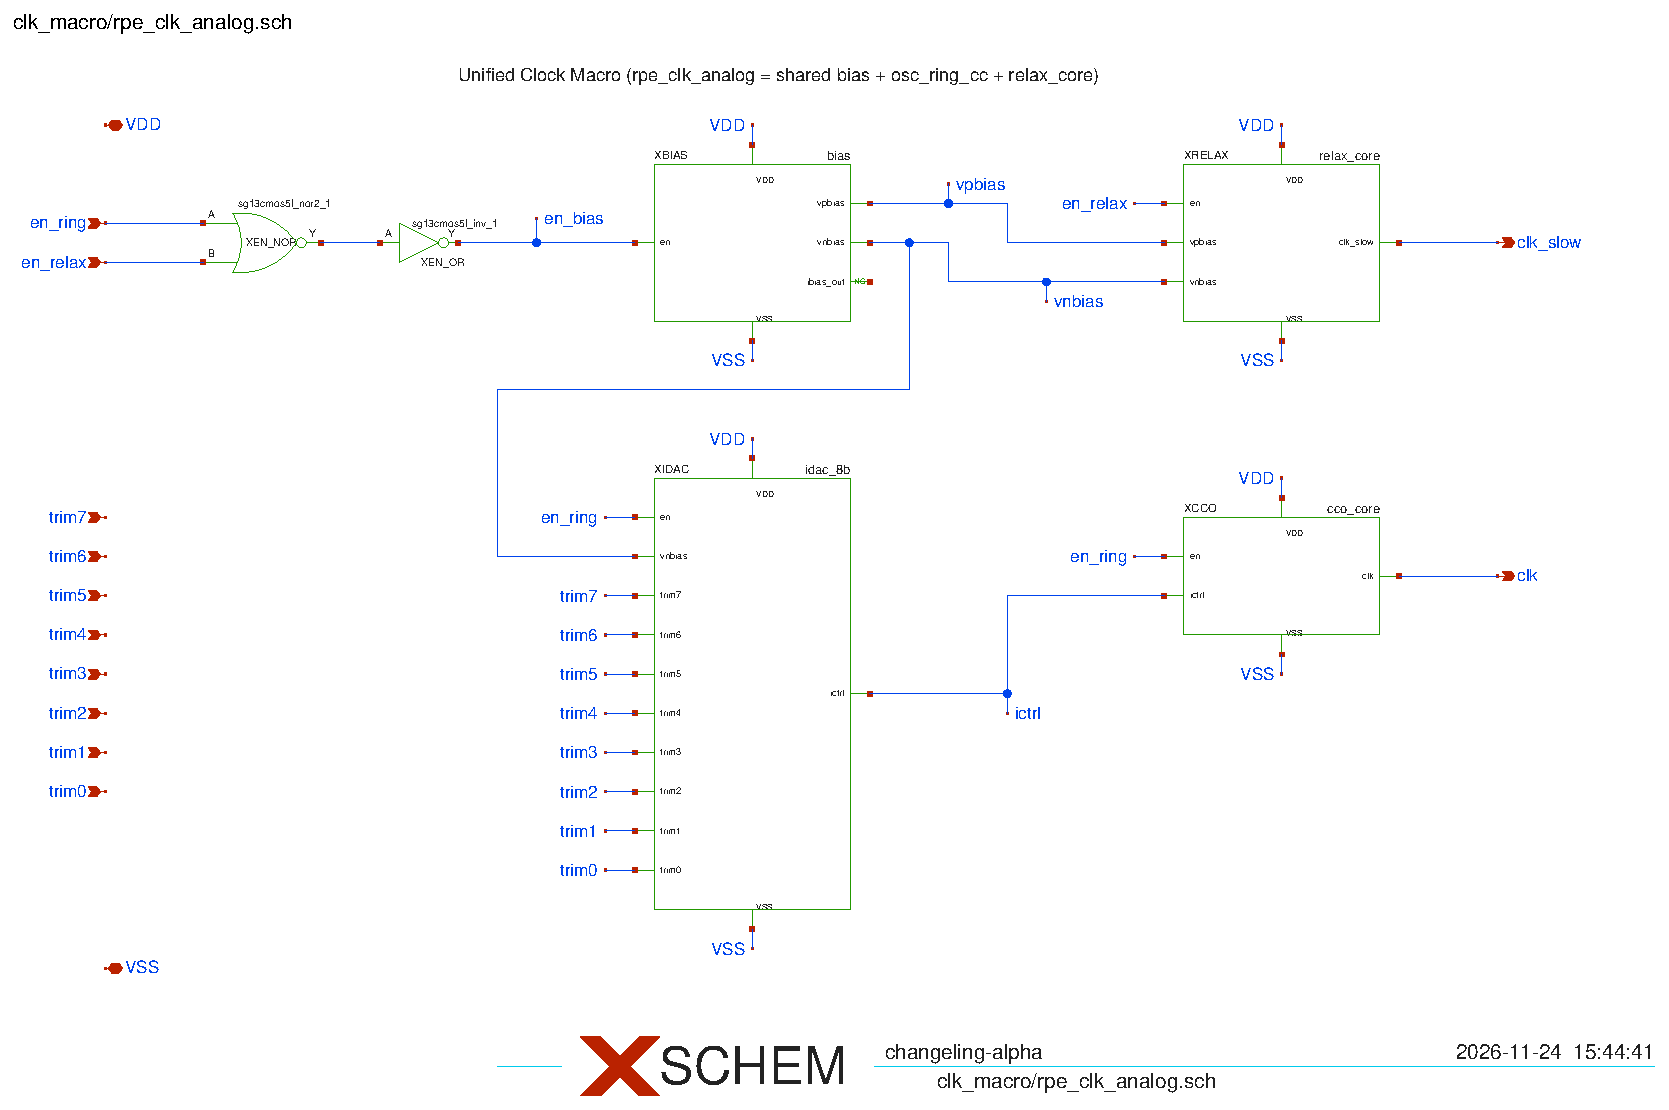
\includegraphics[width=0.90\textwidth]{figures/sch_rpe_clk_analog.pdf}
\caption{Unified top-level schematic of \texttt{rpe\_clk\_analog}.}
\label{fig:sch_top}
\end{figure}

\begin{figure}[H]
\centering
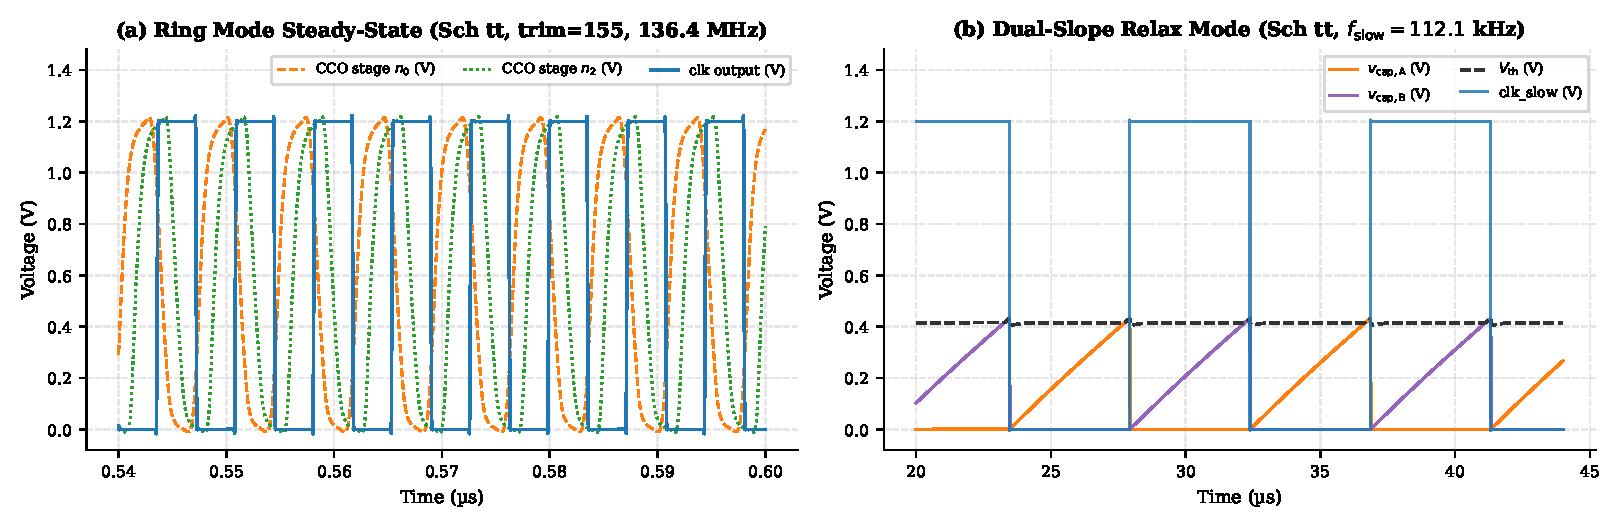
\includegraphics[width=\textwidth]{figures/fig_macro_waveforms.pdf}
\caption{Unified macro schematic transient waveforms (\texttt{tt}, $1.20\text{ V}$, $25\,^\circ\text{C}$): (a) pre-emphasized Ring B output and internal CCO phases $n_0, n_2$ ($136.39\text{ MHz}$); (b) \texttt{relax\_core} dual-slope \texttt{vcap\_a}, \texttt{vcap\_b}, $V_{\text{th}}$, and $112.07\text{ kHz}$ \texttt{clk\_slow}.}
\label{fig:macro_wf}
\end{figure}

\begin{table}[H]
\centering
\caption{Pre-Layout Unified Macro Schematic Matrix (\texttt{clk\_macro\_modes.csv}, all 15 Mode $\times$ Corner Runs).}
\label{tab:macro_modes}
\footnotesize
\setlength{\tabcolsep}{4pt}
\begin{tabular}{@{}lllcccccc@{}}
\toprule
\textbf{Mode} & \textbf{Corner} & \textbf{$V_{DD}$ / Temp} & \textbf{Trim} & \textbf{$f_{\text{ring}}$ (MHz)} & \textbf{Ring Duty} & \textbf{$f_{\text{relax}}$ (kHz)} & \textbf{Relax Duty} & \textbf{$I_{DD}$ / Standby} \\
\midrule
\texttt{standby} & \texttt{tt} & $1.20\text{ V}$ / $25\,^\circ\text{C}$ & 128 & $0.0000$ & --- & $0.000$ & --- & $5.826\text{ nA}$ \\
\texttt{ring\_only} & \texttt{tt} & $1.20\text{ V}$ / $25\,^\circ\text{C}$ & 128 & $120.1297$ & $50.01\%$ & $0.000$ & --- & $64.812\,\mu\text{A}$ \\
\texttt{ring\_only} & \texttt{tt} & $1.20\text{ V}$ / $25\,^\circ\text{C}$ & 155 & $136.3866$ & $49.51\%$ & $0.000$ & --- & $73.437\,\mu\text{A}$ \\
\texttt{sleep\_relax} & \texttt{tt} & $1.20\text{ V}$ / $25\,^\circ\text{C}$ & 155 & $0.0000$ & --- & $112.070$ & $49.96\%$ & $3.999\,\mu\text{A}$ \\
\texttt{both\_active} & \texttt{tt} & $1.20\text{ V}$ / $25\,^\circ\text{C}$ & 155 & $131.2680$ & $48.96\%$ & $111.870$ & $49.99\%$ & $73.538\,\mu\text{A}$ \\
\midrule
\texttt{standby} & \texttt{ss} & $1.08\text{ V}$ / $125\,^\circ\text{C}$ & 128 & $0.0000$ & --- & $0.000$ & --- & $68.497\text{ nA}$ \\
\texttt{ring\_only} & \texttt{ss} & $1.08\text{ V}$ / $125\,^\circ\text{C}$ & 128 & $122.2255$ & $50.06\%$ & $0.000$ & --- & $60.668\,\mu\text{A}$ \\
\texttt{ring\_only} & \texttt{ss} & $1.08\text{ V}$ / $125\,^\circ\text{C}$ & 155 & $136.0396$ & $49.63\%$ & $0.000$ & --- & $67.949\,\mu\text{A}$ \\
\texttt{sleep\_relax} & \texttt{ss} & $1.08\text{ V}$ / $125\,^\circ\text{C}$ & 155 & $0.0000$ & --- & $95.069$ & $49.95\%$ & $4.239\,\mu\text{A}$ \\
\texttt{both\_active} & \texttt{ss} & $1.08\text{ V}$ / $125\,^\circ\text{C}$ & 155 & $131.3715$ & $49.26\%$ & $94.921$ & $49.98\%$ & $65.847\,\mu\text{A}$ \\
\midrule
\texttt{standby} & \texttt{ff} & $1.32\text{ V}$ / $-40\,^\circ\text{C}$ & 128 & $0.0000$ & --- & $0.000$ & --- & $8.168\text{ nA}$ \\
\texttt{ring\_only} & \texttt{ff} & $1.32\text{ V}$ / $-40\,^\circ\text{C}$ & 128 & $128.4131$ & $50.07\%$ & $0.000$ & --- & $80.659\,\mu\text{A}$ \\
\texttt{ring\_only} & \texttt{ff} & $1.32\text{ V}$ / $-40\,^\circ\text{C}$ & 155 & $147.4941$ & $49.77\%$ & $0.000$ & --- & $91.352\,\mu\text{A}$ \\
\texttt{sleep\_relax} & \texttt{ff} & $1.32\text{ V}$ / $-40\,^\circ\text{C}$ & 155 & $0.0000$ & --- & $131.904$ & $49.94\%$ & $4.429\,\mu\text{A}$ \\
\texttt{both\_active} & \texttt{ff} & $1.32\text{ V}$ / $-40\,^\circ\text{C}$ & 155 & $144.2585$ & $51.07\%$ & $131.612$ & $49.98\%$ & $93.950\,\mu\text{A}$ \\
\bottomrule
\end{tabular}
\end{table}

% =============================================================================
% SECTION 4: CUSTOM PHYSICAL LAYOUT
% =============================================================================
\section{Custom Physical Layout \& Compaction}

The compacted \texttt{rpe\_clk\_analog} layout (Figure~\ref{fig:layout_full}) is constructed hierarchically inside a $171.500 \times 137.000\,\mu\text{m}$ PR boundary ($23{,}495.5\,\mu\text{m}^2$, $-42.1\%$ area relative to the initial $236.0 \times 172.0\,\mu\text{m}$ baseline) surrounded by concentric $1.4\,\mu\text{m}$-wide \texttt{Metal4} power rings (outer \texttt{VSS}, inner \texttt{VDD}) stitched with substrate \texttt{ptap1} contacts every $15\,\mu\text{m}$. Four architectural and routing upgrades drove this compaction without sacrificing any active/passive matching rules:
\begin{itemize}
  \item \textbf{Tighter Router Tracks \& Interval Packing (\texttt{NetRouter}):} Reduced \texttt{Metal2}/\texttt{Metal3} routing pitch from $0.72$--$0.80\,\mu\text{m}$ to $0.66\,\mu\text{m}$, tightened standard-cell pin escape gutters to $0.48\,\mu\text{m}$, and enabled interval-packed track reuse (\texttt{pack=True}) so horizontally disjoint nets share horizontal \texttt{Metal2} tracks.
  \item \textbf{Folded 2-Column Floorplan:} Reorganized the top-level placement so the taller $5$-column \texttt{idac\_8b\_lay} ($47.090 \times 121.800\,\mu\text{m}$) occupies the full West column, while \texttt{bias\_lay} + \texttt{cco\_core\_lay} sit side by side along the South-East below \texttt{relax\_core\_lay} in the North-East, separated by a central \texttt{Metal2}/\texttt{Metal3} signal corridor hosting \texttt{en\_or} without empty dead-space islands.
  \item \textbf{Subblock Packing \& Non-Inverting CCO Routing:} Restacked \texttt{idac\_8b\_lay}'s $311$ PMOS current units into $5$ denser columns ($d_y=1.08\,\mu\text{m}$) inside an L-shaped \texttt{NWell}, consolidated comparator stacks and bus lanes in \texttt{relax\_core\_lay} ($-33.2\%$, $N_x=8$ \texttt{SVaricap}), compacted \texttt{comp\_lay} by $-35.8\%$, and shrank \texttt{cco\_core\_lay} by $-29.4\%$ ($2.4\times 2.4\,\mu\text{m}$ \texttt{cap\_cmomf}) while ordering feedback loops non-monotonically (\texttt{0,2,4,1,3}) so adjacent parallel tracks carry same-polarity signals without $2\times$ Miller capacitance multiplication.
\end{itemize}

\begin{figure}[H]
\centering
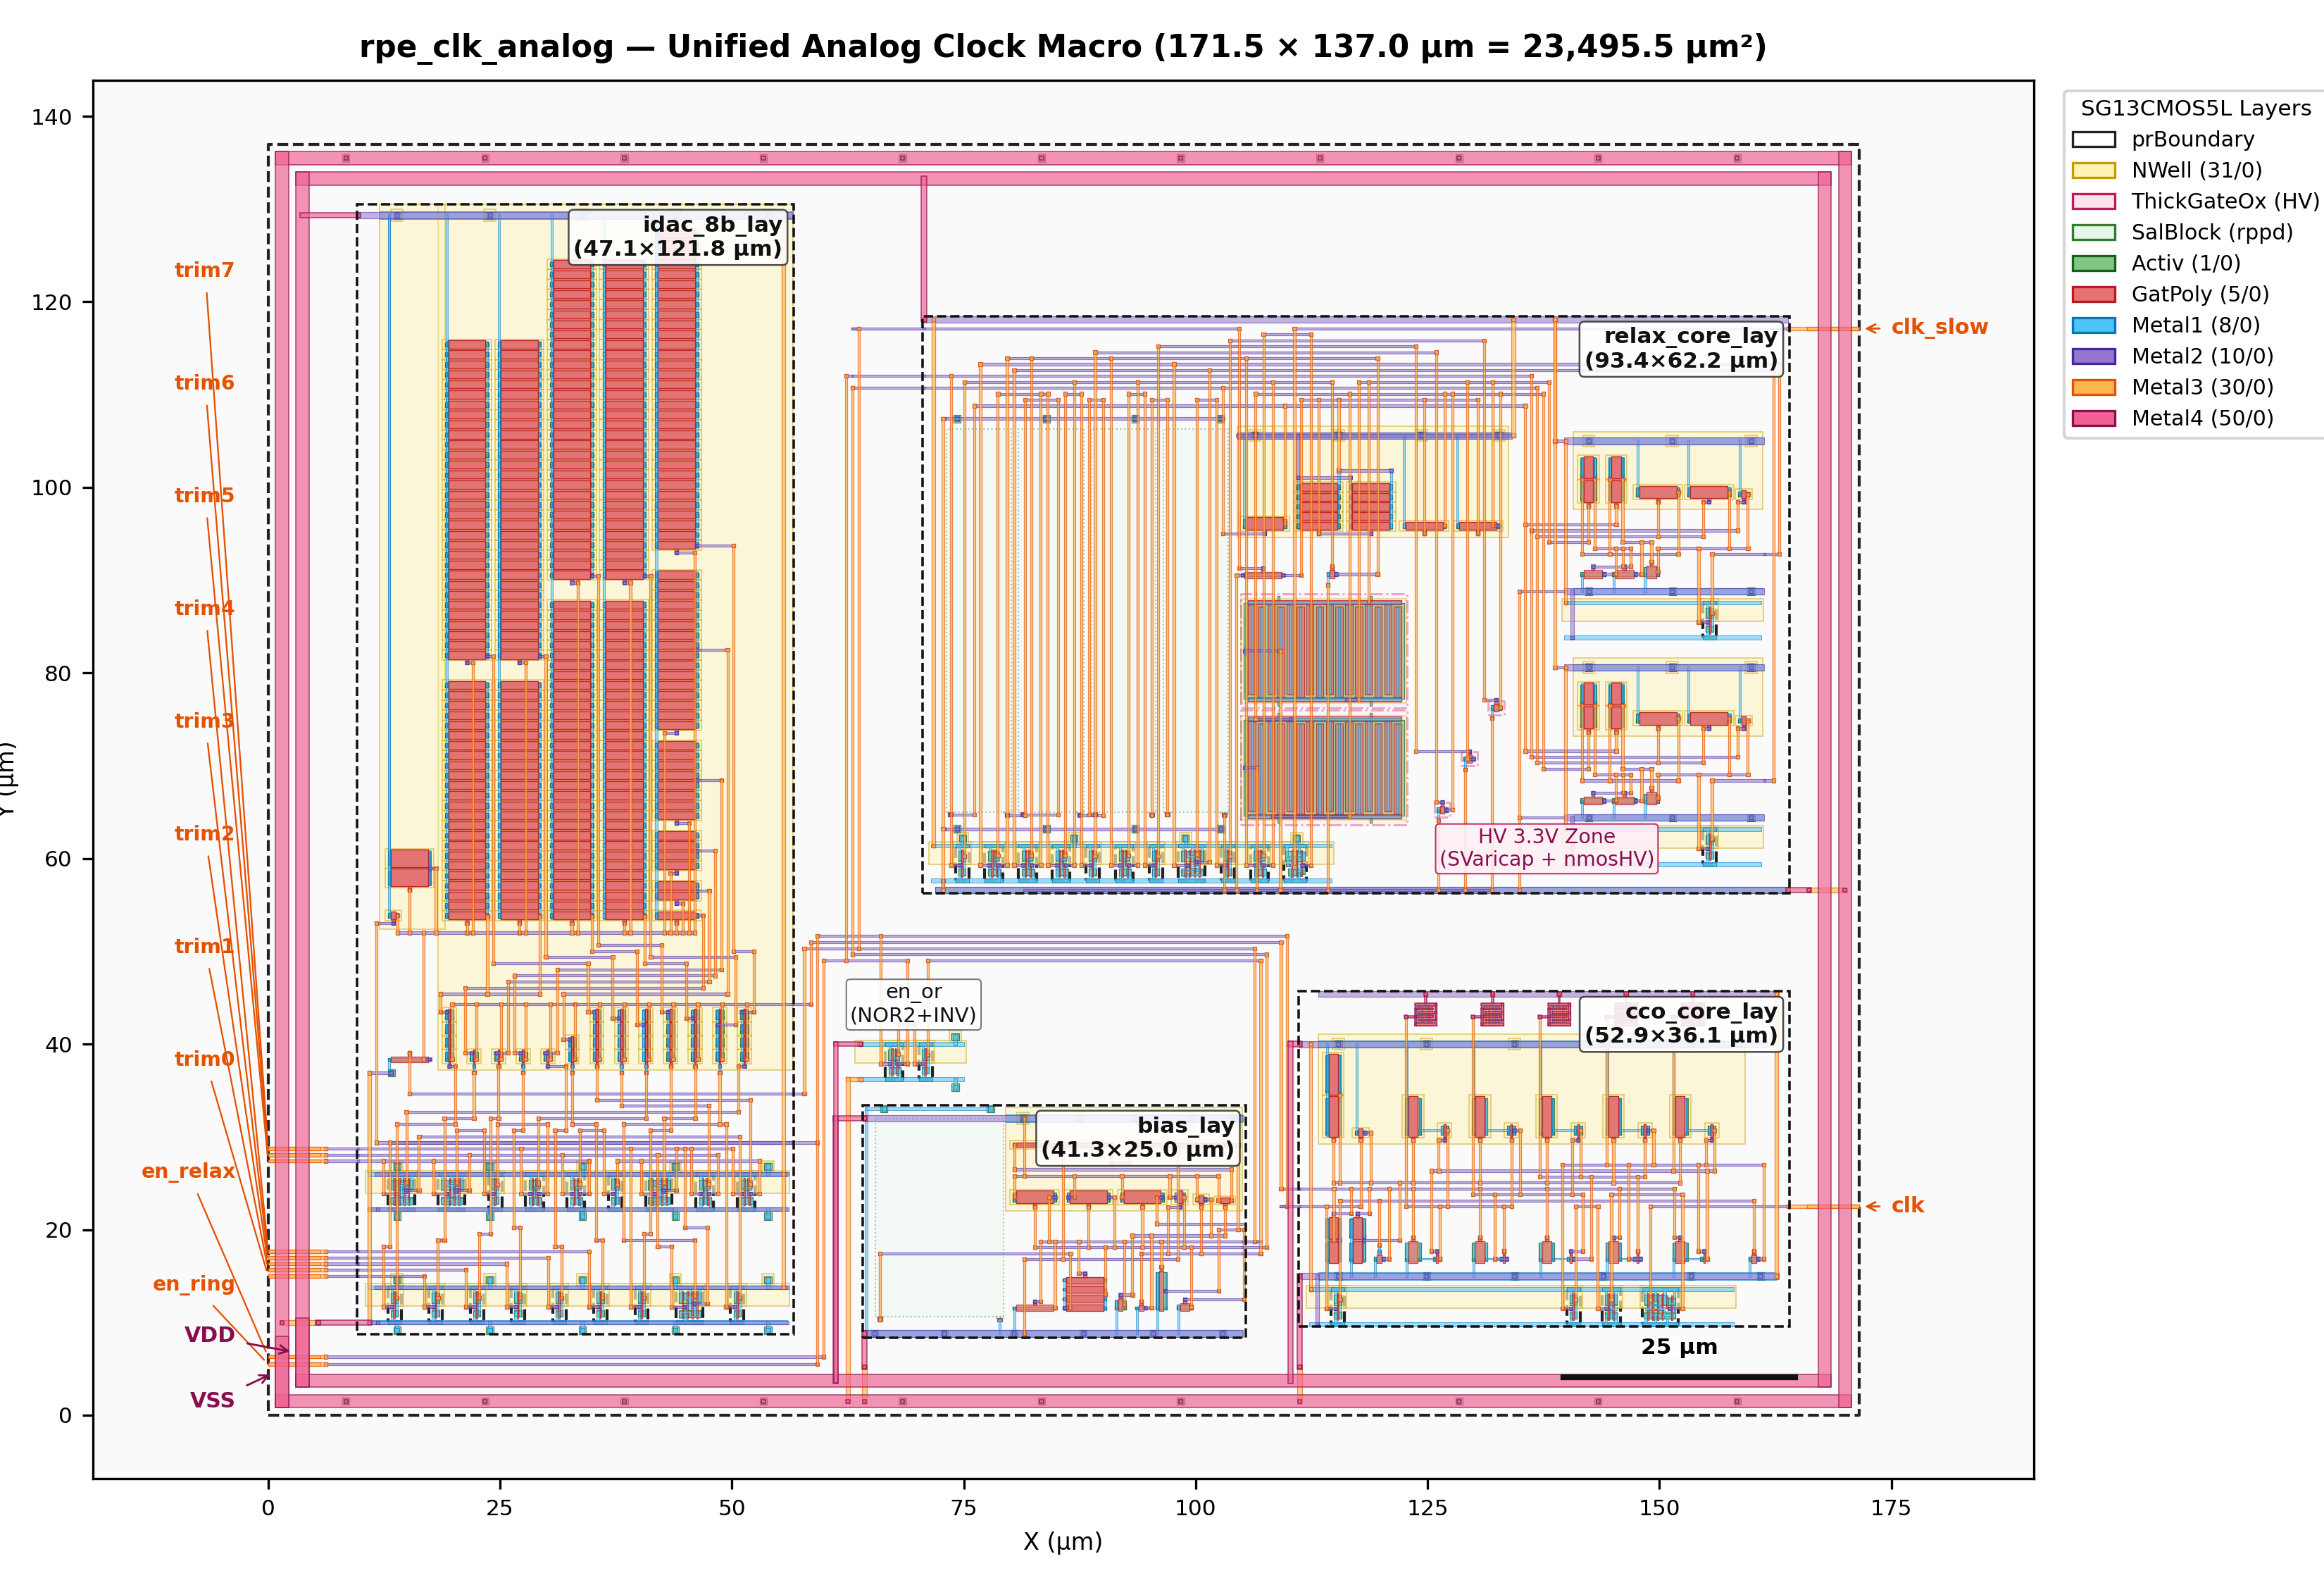
\includegraphics[width=\textwidth]{figures/fig_layout_full.png}
\caption{Compacted physical layout of \texttt{rpe\_clk\_analog} ($171.500 \times 137.000\,\mu\text{m} = 23{,}495.5\,\mu\text{m}^2$, $-42.1\%$), showing dual \texttt{Metal4} power rings, all four analog subblocks, \texttt{en\_or}, the $3.3\text{ V}$ HV region, and all $14$ boundary pins. (Zoomable 6-page vector PDF in \texttt{analog/results/layouts.pdf}.)}
\label{fig:layout_full}
\end{figure}

Key physical isolation measures preserved across compaction (Figure~\ref{fig:layout_zooms}) include the L-shaped \texttt{NWell} excluding \texttt{MN\_DIV} in \texttt{idac\_8b\_lay}, contiguous \texttt{Metal3} inter-block \texttt{VSS} underpasses beneath the \texttt{Metal4} \texttt{VDD} ring, and strict spatial separation in \texttt{relax\_core\_lay} between the four left-hand \texttt{rppd} segments, the central $3.3\text{ V}$ \texttt{ThickGateOx} \texttt{SVaricap}/\texttt{nmosHV} island, and the two stacked \texttt{comp\_lay} comparators on the right.

\begin{figure}[H]
\centering
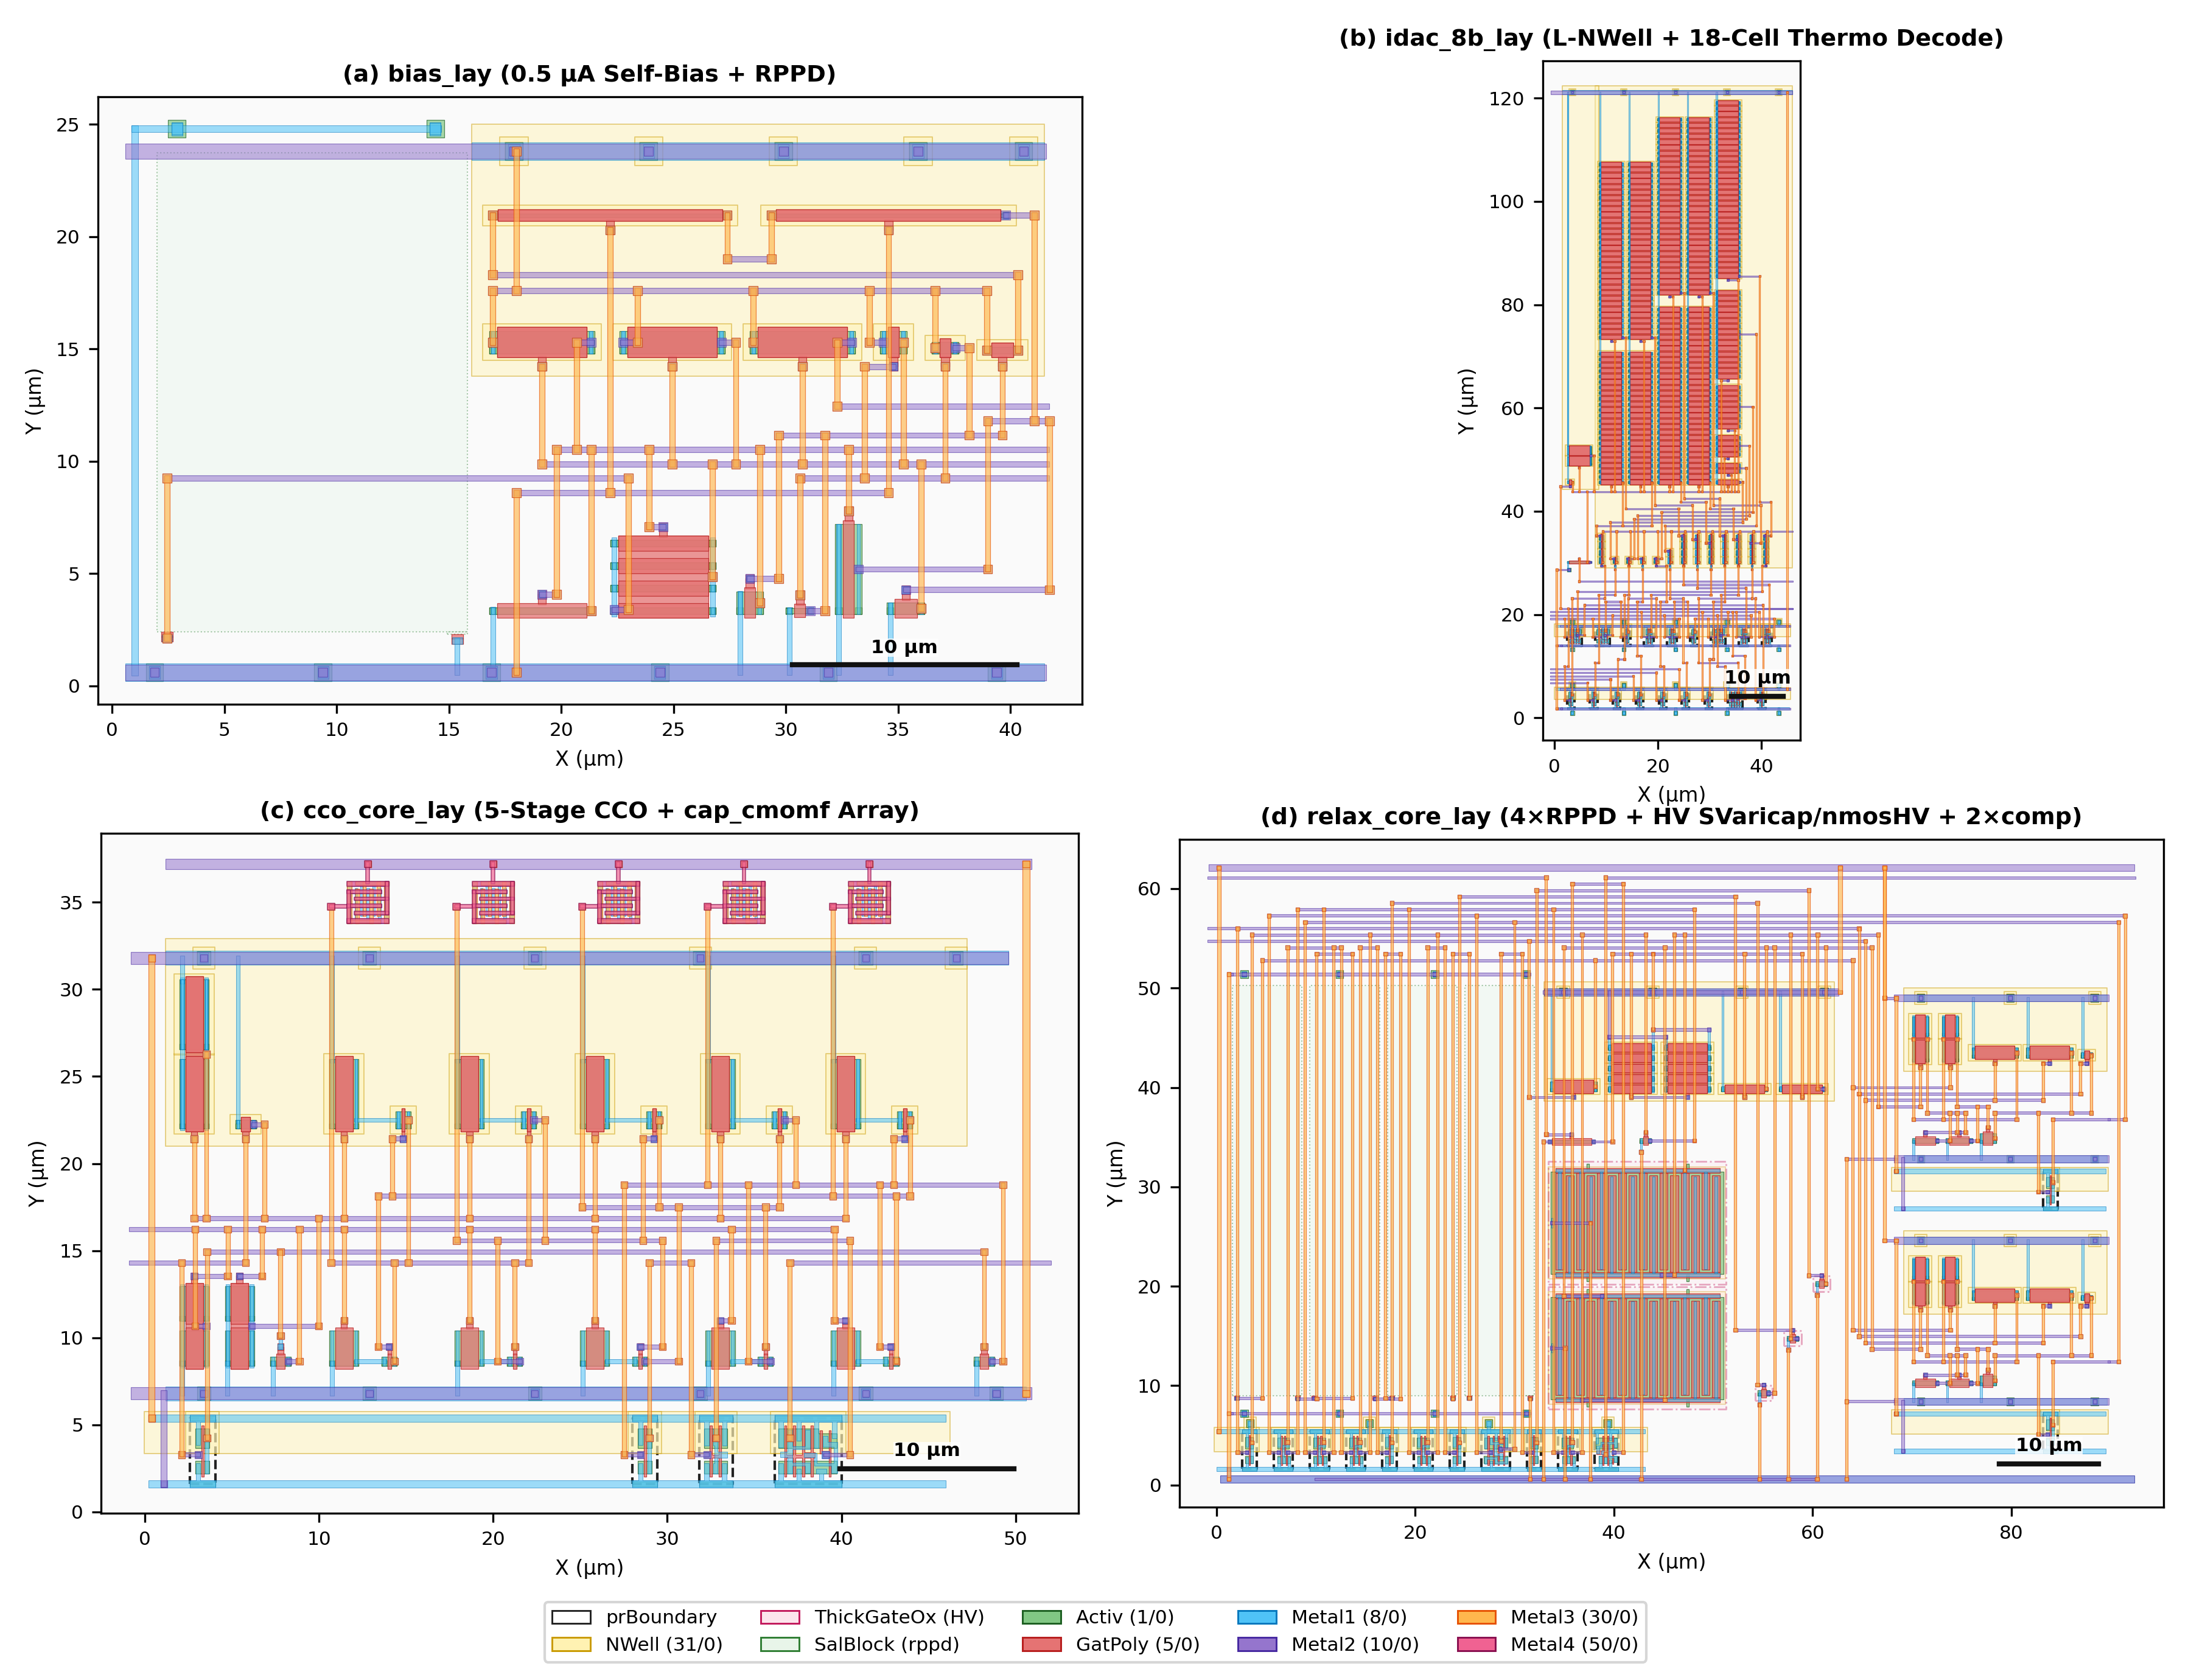
\includegraphics[width=\textwidth]{figures/fig_layout_zooms.png}
\caption{Detailed layout views of the four compacted core subblocks: (a) \texttt{bias\_lay}, (b) \texttt{idac\_8b\_lay}, (c) \texttt{cco\_core\_lay}, and (d) \texttt{relax\_core\_lay}.}
\label{fig:layout_zooms}
\end{figure}

\begin{table}[H]
\centering
\caption{Before-vs.-After Compaction Summary: Physical Dimensions \& Area Reduction (\texttt{drc\_summary.txt}).}
\label{tab:area_breakdown}
\footnotesize
\setlength{\tabcolsep}{4pt}
\begin{tabularx}{\textwidth}{@{}lrrrrr >{\raggedright\arraybackslash}X@{}}
\toprule
\textbf{Cell Name} & \textbf{v1 Area ($\mu\text{m}^2$)} & \textbf{v2 Width ($\mu\text{m}$)} & \textbf{v2 Height ($\mu\text{m}$)} & \textbf{v2 Area ($\mu\text{m}^2$)} & \textbf{$\Delta$ Area} & \textbf{Dominant Structures} \\
\midrule
\texttt{bias\_lay} & $1{,}341.2$ & $41.340$ & $25.040$ & $1{,}035.2$ & $-22.8\%$ & $1\times\text{rppd}$ ($b=19$), self-bias + startup \\
\texttt{idac\_8b\_lay} & $8{,}365.0$ & $47.090$ & $121.800$ & $5{,}735.6$ & $-31.4\%$ & $18$ stdcells, L-\texttt{NWell}, $311\times$ PMOS units \\
\texttt{cco\_core\_lay} & $2{,}708.8$ & $52.940$ & $36.120$ & $1{,}912.2$ & $-29.4\%$ & $5\times 2.4\,\mu\text{m}$ CMOMF, non-inv.\ loop, $4$ stdcells \\
\texttt{comp\_lay} ($2\times$) & $766.5$ & $21.960$ & $22.420$ & $492.3$ & $-35.8\%$ & Diff.\ PMOS pair, NMOS mirror, \texttt{inv\_1} \\
\texttt{relax\_core\_lay} & $8{,}706.1$ & $93.440$ & $62.220$ & $5{,}813.8$ & $-33.2\%$ & $4\times\text{rppd}$, $2\times\text{SVaricap}$, $3\times\text{nmosHV}$, $11$ stdcells \\
\midrule
\textbf{\texttt{rpe\_clk\_analog} Top} & $\mathbf{40{,}592.0}$ & $\mathbf{171.500}$ & $\mathbf{137.000}$ & $\mathbf{23{,}495.5}$ & $\mathbf{-42.1\%}$ & 2-col.\ floorplan, dual \texttt{M4} ring, \texttt{en\_or} \\
\bottomrule
\end{tabularx}
\end{table}

% =============================================================================
% SECTION 5: PHYSICAL VERIFICATION SIGN-OFF & PEX
% =============================================================================
\section{Physical Verification Sign-Off (DRC, LVS \& Magic PEX)}
\label{sec:signoff}

\subsection{KLayout DRC \& Strict-Port LVS Sign-Off}
Table~\ref{tab:signoff} summarizes KLayout DRC and LVS sign-off on the final PEX-re-centered and compacted \texttt{rpe\_clk\_analog.gds}. Both the standard DRC rule deck (\texttt{tables=main}, $3.82\text{ s}$) and the combined main+antenna check (\texttt{tables="main antenna"}, $6.94\text{ s}$) pass with zero violations. Strict-port LVS matches all $14$ top-level pins, $117$ combined nets, and $211$ combined active/passive devices ($580$ pre-combination layout devices) in $1.75\text{ s}$.

\begin{table}[H]
\centering
\caption{Physical Verification Sign-Off Summary (KLayout 0.30.12, \texttt{ihp-sg13cmos5l}).}
\label{tab:signoff}
\footnotesize
\setlength{\tabcolsep}{4pt}
\begin{tabularx}{\textwidth}{@{}ll >{\raggedright\arraybackslash}X l@{}}
\toprule
\textbf{Check} & \textbf{Configuration} & \textbf{Scope Verified} & \textbf{Result} \\
\midrule
DRC (\texttt{main}) & \texttt{ihp-sg13cmos5l.drc}, \texttt{tables=main} & FEOL, BEOL, OFFGRID, ANGLE, PIN, FORBIDDEN (\texttt{M5/TM2}), CONNECTIVITY & \textbf{\textcolor{PassGreen}{0 violations}} \\
DRC (\texttt{antenna}) & \texttt{ihp-sg13cmos5l.drc}, \texttt{tables="main antenna"} & Metal1--Metal4 \& Via1--Via3 antenna ratios + full main ruleset & \textbf{\textcolor{PassGreen}{0 violations}} \\
LVS & \texttt{sg13cmos5l.lvs}, strict port mode & $83\times\texttt{sg13\_lv\_nmos}$, $116\times\texttt{sg13\_lv\_pmos}$, $3\times\texttt{sg13\_hv\_nmos}$, $2\times\texttt{sg13\_hv\_svaricap}$, $5\times\texttt{cap\_cmomf}$, $2\times\texttt{rppd}$ ($117$ nets, $14$ pins) & \textbf{\textcolor{PassGreen}{MATCH}} \\
\bottomrule
\end{tabularx}
\end{table}

\paragraph{Engineering Note on IHP PDK LVS Netlist Preparation.}
Two PDK-level \texttt{xschem}-vs.-KLayout netlist conventions were bridged cleanly in \texttt{clk\_macro/Makefile} without altering any GDS geometry or \texttt{SG13\_dev} PCells:
\begin{enumerate}
  \item \textbf{Standard-Cell Subcircuit Primitives:} \texttt{sg13cmos5l\_stdcell.cdl} (\texttt{MN0}/\texttt{MP0} MOSFET primitives) is appended to the LVS netlist instead of the simulation \texttt{.spice} file (whose \texttt{XN0}/\texttt{XP0} calls are treated as subcircuit calls by KLayout's netlist reader).
  \item \textbf{\texttt{rppd.sym} Parameter Extraction Parity:} Official \texttt{xschem} \texttt{rppd.sym} omits \texttt{ps=0.18u} in its \texttt{lvs\_format} string while \texttt{custom\_devices.lvs} compares \texttt{ps} with zero tolerance, and IHP's \texttt{rppd} layout PCell and \texttt{custom\_extractor.lvs} include endcap/bend length (\texttt{contactpush} and \texttt{length+=width}), extracting $l=21.125\,\mu\text{m}$ for drawn $w=0.5\,\mu\text{m}, l=20.0\,\mu\text{m}, b=19$ and $l=41.055\,\mu\text{m}$ for drawn $w=0.5\,\mu\text{m}, l=40.0\,\mu\text{m}, b=9$. The \texttt{lvs\_netlist} target normalizes those two schematic resistor strings to match IHP's reference \texttt{rppd.cdl} unit-test convention.
\end{enumerate}

\subsection{True Hierarchical Magic 8.3.677 PEX \& Post-Layout Closure}
\label{sec:pex}
Post-layout RC/C parasitic extraction was performed on the re-centered \texttt{rpe\_clk\_analog.gds} using Magic 8.3.677 (\texttt{ihp-sg13cmos5l} techfile with \texttt{extract all}, \texttt{ext2spice lvs}, and \texttt{cthresh 0.01}) via \texttt{clk\_macro/extract\_pex.py}. Crucially, full subcircuit hierarchy was preserved (omitting \texttt{ext2spice hierarchy off}) because flattening during \texttt{ext2spice} causes Magic to lump all drain/source diffusion areas and perimeters onto a single transistor per shared net. Paired half-varicap regions (\texttt{N0}/\texttt{N1}) inside \texttt{.subckt SVaricap} were reassembled into single PDK \texttt{sg13\_hv\_svaricap} subcircuit calls ($N_x = 8$, $w_{\text{avg}} \approx 9.77\,\mu\text{m}, l = 0.8\,\mu\text{m}$), \texttt{.subckt rppd} was renamed \texttt{rppd\_cell} to avoid shadowing the PDK resistor model, and \texttt{.options rshunt=1e12} ($10^{14}\,\Omega$ for standby DC \texttt{.op}) was applied so purely capacitive dummy nodes inside extracted \texttt{rppd} subcells initialize without DC matrix singularity.

Across the re-centered hierarchy ($37$ subcircuits containing $103\times\texttt{sg13\_lv\_nmos}$, $462\times\texttt{sg13\_lv\_pmos}$, $3\times\texttt{sg13\_hv\_nmos}$, $5\times\texttt{rppd}$ segments, and $2\times\texttt{sg13\_hv\_svaricap}$), Magic extracts $\mathbf{3{,}607}$ \textbf{capacitors} ($\ge 0.01\text{ fF}$) totaling $\mathbf{1{,}334.46\text{ fF}}$ ($\mathbf{1.334\text{ pF}}$): $310.55\text{ fF}$ to ground/substrate and $1{,}023.90\text{ fF}$ inter-node coupling (including the $5$ downsized $2.4\times 2.4\,\mu\text{m}$ \texttt{cap\_cmomf} arrays). Table~\ref{tab:pex_vs_sch} and Figure~\ref{fig:pex_comp} compare schematic and Magic PEX results across all $15$ PVT runs plus \texttt{trim=255} corner headroom.

\begin{table}[H]
\centering
\caption{Schematic vs.\ Hierarchical Magic PEX Verification Matrix (\texttt{clk\_macro\_modes.csv} vs.\ \texttt{clk\_macro\_pex.csv} / \texttt{clk\_macro\_pex\_trim.csv}).}
\label{tab:pex_vs_sch}
\scriptsize
\setlength{\tabcolsep}{3.0pt}
\begin{tabular}{@{}llccccccccc@{}}
\toprule
\textbf{Mode} & \textbf{Cor.} & \textbf{Trim} & \textbf{Sch.\ Ring} & \textbf{PEX Ring} & \textbf{$\Delta_{\text{ring}}$} & \textbf{Sch.\ Relax} & \textbf{PEX Relax} & \textbf{Sch.\ $I_{DD}$} & \textbf{PEX $I_{DD}$} \\
 & & & \textbf{(MHz)} & \textbf{(MHz)} & & \textbf{(kHz)} & \textbf{(kHz)} & & \\
\midrule
\texttt{standby} & \texttt{tt} & 128 & 0.0000 & 0.0000 & --- & 0.000 & 0.000 & $5.826\text{ nA}$ & $6.052\text{ nA}$ \\
\texttt{ring\_only} & \texttt{tt} & 128 & $120.1297$ & $52.7764$ & $-56.1\%$ & 0.000 & 0.000 & $64.812\,\mu\text{A}$ & $54.908\,\mu\text{A}$ \\
\texttt{ring\_only} & \texttt{tt} & 155 & $136.3866$ & $\mathbf{59.9185}$ & $-56.1\%$ & 0.000 & 0.000 & $73.437\,\mu\text{A}$ & $61.501\,\mu\text{A}$ \\
\texttt{ring\_only} (max) & \texttt{tt} & 255 & $193.6264$ & $83.7710$ & $-56.7\%$ & 0.000 & 0.000 & $100.45\,\mu\text{A}$ & $86.267\,\mu\text{A}$ \\
\texttt{sleep\_relax} & \texttt{tt} & 155 & 0.0000 & 0.0000 & --- & $112.070$ & $\mathbf{98.538}$ & $3.999\,\mu\text{A}$ & $4.147\,\mu\text{A}$ \\
\texttt{both\_active} & \texttt{tt} & 155 & $131.2680$ & $57.0776$ & $-56.5\%$ & $111.870$ & $99.018$ & $73.538\,\mu\text{A}$ & $62.539\,\mu\text{A}$ \\
\midrule
\texttt{standby} & \texttt{ss} & 128 & 0.0000 & 0.0000 & --- & 0.000 & 0.000 & $68.497\text{ nA}$ & $68.684\text{ nA}$ \\
\texttt{ring\_only} & \texttt{ss} & 128 & $122.2255$ & $52.9796$ & $-56.7\%$ & 0.000 & 0.000 & $60.668\,\mu\text{A}$ & $51.182\,\mu\text{A}$ \\
\texttt{ring\_only} & \texttt{ss} & 155 & $136.0396$ & $59.0958$ & $-56.6\%$ & 0.000 & 0.000 & $67.949\,\mu\text{A}$ & $57.635\,\mu\text{A}$ \\
\texttt{ring\_only} (max) & \texttt{ss} & 255 & $179.2217$ & $78.0774$ & $-56.4\%$ & 0.000 & 0.000 & $91.22\,\mu\text{A}$ & $80.316\,\mu\text{A}$ \\
\texttt{sleep\_relax} & \texttt{ss} & 155 & 0.0000 & 0.0000 & --- & $95.069$ & $83.597$ & $4.239\,\mu\text{A}$ & $4.212\,\mu\text{A}$ \\
\texttt{both\_active} & \texttt{ss} & 155 & $131.3715$ & $56.5355$ & $-57.0\%$ & $94.921$ & $83.817$ & $65.847\,\mu\text{A}$ & $58.204\,\mu\text{A}$ \\
\midrule
\texttt{standby} & \texttt{ff} & 128 & 0.0000 & 0.0000 & --- & 0.000 & 0.000 & $8.168\text{ nA}$ & $8.408\text{ nA}$ \\
\texttt{ring\_only} & \texttt{ff} & 128 & $128.4131$ & $\mathbf{58.5099}$ & $-54.4\%$ & 0.000 & 0.000 & $80.659\,\mu\text{A}$ & $69.790\,\mu\text{A}$ \\
\texttt{ring\_only} & \texttt{ff} & 155 & $147.4941$ & $66.9184$ & $-54.6\%$ & 0.000 & 0.000 & $91.352\,\mu\text{A}$ & $78.351\,\mu\text{A}$ \\
\texttt{ring\_only} (max) & \texttt{ff} & 255 & $218.5653$ & $96.8895$ & $-55.7\%$ & 0.000 & 0.000 & $129.83\,\mu\text{A}$ & $110.166\,\mu\text{A}$ \\
\texttt{sleep\_relax} & \texttt{ff} & 155 & 0.0000 & 0.0000 & --- & $131.904$ & $115.504$ & $4.429\,\mu\text{A}$ & $5.109\,\mu\text{A}$ \\
\texttt{both\_active} & \texttt{ff} & 155 & $144.2585$ & $64.6329$ & $-55.2\%$ & $131.612$ & $116.012$ & $93.950\,\mu\text{A}$ & $80.419\,\mu\text{A}$ \\
\bottomrule
\end{tabular}
\end{table}

\begin{figure}[H]
\centering
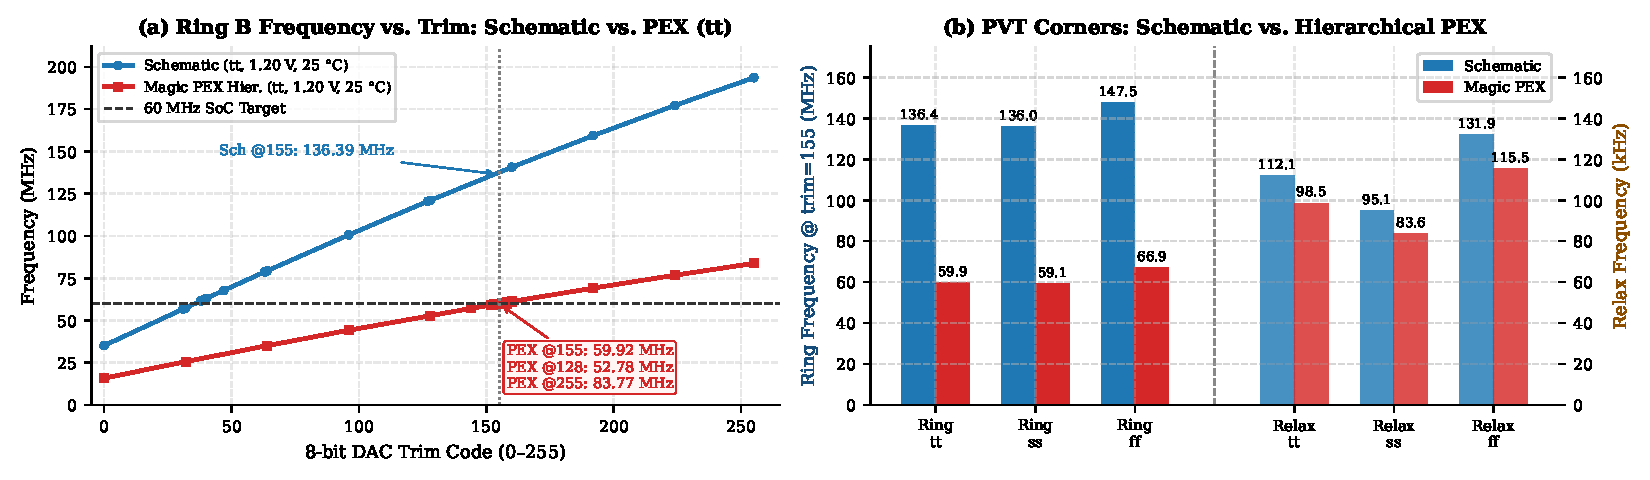
\includegraphics[width=0.67\textwidth]{figures/fig_pex_comparison.pdf}
\vspace{-4pt}
\caption{Post-layout Magic PEX vs.\ schematic comparison: (a) \texttt{tt} Ring B tuning linearity (PEX \texttt{trim} $0$--$255$ spans $15.84$--$83.77\text{ MHz}$, hitting $59.92\text{ MHz}$ at \texttt{trim=155}); (b) PVT corner summary across \texttt{ring\_only} (\texttt{trim=155}) and \texttt{sleep\_relax}.}
\label{fig:pex_comp}
\end{figure}

\vspace{-6pt}
\paragraph{PEX Re-Centering Outcome \& Design Closure.}
{\small In the initial compacted layout (before re-centering), $3.6\times 3.6\,\mu\text{m}$ CMOMF loading plus inverting inter-stage Miller coupling capped post-layout \texttt{ring\_only} at $45.01\text{ MHz}$ (\texttt{tt}, \texttt{trim=255}) and shifted \texttt{sleep\_relax} to $88.58\text{ kHz}$. Applying the three co-designed physical/circuit updates achieved full PEX sign-off closure:
\begin{enumerate}\setlength{\itemsep}{1pt}\setlength{\parskip}{0pt}\setlength{\topsep}{0pt}
  \item \textbf{Ring Oscillator $60\text{ MHz}$ Closure Across PVT:} Downsizing \texttt{cap\_cmomf} to $2.4\times 2.4\,\mu\text{m}$, boosting \texttt{MP\_IN} drive $1.33\times$ ($w=1.5\,\mu\text{m}$), and routing feedback loops non-monotonically (\texttt{0,2,4,1,3}) reduced total extracted macro capacitance ($1{,}467.10\text{ fF} \to 1{,}334.46\text{ fF}$) and doubled stage bandwidth. Magic PEX now crosses $60\text{ MHz}$ right at mid-trim (\texttt{trim=155}: $59.92\text{ MHz}$, $48.74\%$ duty, $61.50\,\mu\text{A}$) with $+30.1\%$ upper headroom in \texttt{ss} ($78.08\text{ MHz}$ at \texttt{255}) while still holding boot \texttt{trim=128} $\le 60\text{ MHz}$ across \texttt{tt}/\texttt{ss}/\texttt{ff} ($52.78 / 52.98 / 58.51\text{ MHz}$).
  \item \textbf{Relaxation Oscillator Re-Centering:} Trimming \texttt{SVaricap} from $N_x=9$ to $N_x=8$ compensated the $\sim 29\text{ fF}$ comparator/routing load, raising post-layout \texttt{sleep\_relax} from $88.58\text{ kHz}$ to $98.54\text{ kHz}$ (\texttt{tt}, $50.02\%$ duty, $4.15\,\mu\text{A}$), with negligible \texttt{both\_active} interference ($+0.49\%$ shift on \texttt{clk\_slow}).
  \item \textbf{Ultra-Low Leakage Integrity:} Post-layout standby leakage remains practically identical to schematic ($6.05\text{ nA}$ \texttt{tt}, $68.68\text{ nA}$ \texttt{ss} $125\,^\circ\text{C}$, $8.41\text{ nA}$ \texttt{ff}).
\end{enumerate}}

% =============================================================================
% SECTION 6: SOC INTEGRATION
% =============================================================================
\vspace{-6pt}
\section{Digital SoC Integration (\texttt{LEF}, \texttt{OBS} \& \texttt{Verilog})}

The hardened macro exports a standard Cadence LEF 5.7 abstract (\texttt{rpe\_clk\_analog.lef}, \texttt{CLASS BLOCK}, \texttt{SYMMETRY X Y R90}) and a Yosys/OpenROAD synthesis blackbox (\texttt{rpe\_clk\_analog.v}). All digital signal ports lie on \texttt{Metal3} at the West ($X=0$) and East ($X=171.500\,\mu\text{m}$) edges on a clean $\ge 0.66\,\mu\text{m}$ track pitch, while \texttt{VDD}/\texttt{VSS} rails expose \texttt{Metal4} ports for top-level PDN strapping. Routing obstructions (\texttt{OBS}) block \texttt{Metal1}, \texttt{Metal2}, and \texttt{Metal4} across the entire macro ($0..171.500 \times 0..137.000\,\mu\text{m}$) and block \texttt{Metal3} internally over $X=5.800..165.700\,\mu\text{m}$, leaving $5.8\,\mu\text{m}$ East/West pin-access corridors open to the digital router.

\begin{table}[H]
\centering
\vspace{-4pt}
\caption{Exact Compacted \texttt{rpe\_clk\_analog.lef} Pin Abstract (\texttt{SIZE 171.500 BY 137.000}).}
\label{tab:lef_pins}
\scriptsize
\setlength{\tabcolsep}{4pt}
\renewcommand{\arraystretch}{0.72}
\begin{tabular}{@{}llllll@{}}
\toprule
\textbf{Pin} & \textbf{Direction} & \textbf{Use} & \textbf{Layer} & \textbf{RECT ($x_1\ y_1\ x_2\ y_2$, $\mu\text{m}$)} & \textbf{SoC \texttt{rclock} Connection} \\
\midrule
\texttt{VDD} & \texttt{INOUT} & \texttt{POWER} & \texttt{Metal4} & \texttt{3.000 3.000 4.400 10.500} & Core $1.2\text{ V}$ power grid \\
\texttt{VSS} & \texttt{INOUT} & \texttt{GROUND} & \texttt{Metal4} & \texttt{0.800 0.800 2.200 8.500} & Core $0\text{ V}$ ground grid \\
\texttt{en\_ring} & \texttt{INPUT} & \texttt{SIGNAL} & \texttt{Metal3} & \texttt{0.000 5.320 5.600 5.680} & Active-high fast ring enable \\
\texttt{en\_relax} & \texttt{INPUT} & \texttt{SIGNAL} & \texttt{Metal3} & \texttt{0.000 6.120 5.600 6.480} & Active-high slow relax enable \\
\texttt{trim0} & \texttt{INPUT} & \texttt{SIGNAL} & \texttt{Metal3} & \texttt{0.000 14.820 5.600 15.180} & \texttt{trim[0]} (LSB, binary) \\
\texttt{trim1} & \texttt{INPUT} & \texttt{SIGNAL} & \texttt{Metal3} & \texttt{0.000 15.480 5.600 15.840} & \texttt{trim[1]} \\
\texttt{trim2} & \texttt{INPUT} & \texttt{SIGNAL} & \texttt{Metal3} & \texttt{0.000 16.140 5.600 16.500} & \texttt{trim[2]} \\
\texttt{trim3} & \texttt{INPUT} & \texttt{SIGNAL} & \texttt{Metal3} & \texttt{0.000 16.800 5.600 17.160} & \texttt{trim[3]} \\
\texttt{trim4} & \texttt{INPUT} & \texttt{SIGNAL} & \texttt{Metal3} & \texttt{0.000 17.460 5.600 17.820} & \texttt{trim[4]} \\
\texttt{trim5} & \texttt{INPUT} & \texttt{SIGNAL} & \texttt{Metal3} & \texttt{0.000 27.220 5.600 27.580} & \texttt{trim[5]} (MSB thermo bit 0) \\
\texttt{trim6} & \texttt{INPUT} & \texttt{SIGNAL} & \texttt{Metal3} & \texttt{0.000 27.880 5.600 28.240} & \texttt{trim[6]} (MSB thermo bit 1) \\
\texttt{trim7} & \texttt{INPUT} & \texttt{SIGNAL} & \texttt{Metal3} & \texttt{0.000 28.540 5.600 28.900} & \texttt{trim[7]} (MSB thermo bit 2) \\
\texttt{clk} & \texttt{OUTPUT} & \texttt{SIGNAL} & \texttt{Metal3} & \texttt{165.900 22.320 171.500 22.680} & Fast system clock output \\
\texttt{clk\_slow} & \texttt{OUTPUT} & \texttt{SIGNAL} & \texttt{Metal3} & \texttt{165.900 116.940 171.500 117.300} & Always-on/sleep slow clock \\
\bottomrule
\end{tabular}
\end{table}

\begin{lstlisting}[basicstyle=\ttfamily\scriptsize,aboveskip=0pt,belowskip=0pt,caption={Verilog synthesis blackbox view (\texttt{analog/clk\_macro/layout/rpe\_clk\_analog.v}).}]
// Blackbox stub for unified custom analog clock macro (rpe_clk_analog)
(* blackbox *)
module rpe_clk_analog (
    inout  wire       VDD,
    inout  wire       VSS,
    input  wire       en_ring,
    input  wire       en_relax,
    input  wire [7:0] trim,
    output wire       clk,
    output wire       clk_slow
);
endmodule
\end{lstlisting}

\end{document}
